\status{review}
\chapter{Search for X17}
\begin{refsection}
\label{ch:X17}
{\itshape After the recent publications from the ATOMKI collaboration, the so-called X17 anomaly piqued the interest of the community. The flexibility of the MEG II apparatus allows for a variety of exotic searches and the collaboration deemed of interest searching for this anomaly in an uncorrelated way.
The chapter starts with a recap of the previous searches and then moves to the description of this search in MEG II: setup used, simulations developed, data acquisition, and data analysis.}

\status{review}
\section{ATOMKI and the X17 `anomaly'}
    In recent years, the nuclear reaction \ce{^7Li(p,\e,\Ae)^8Be} peaked the physics community's interest.
    The reason is, in 2016 the Atomki laboratory reported an excess in the angular distribution of the pairs $\e \Ae$ coming from the Internal Pair Creation (IPC) \cite{X17:results:2017}.
    The significance found was $\approx7\sigma$ and similar results were later obtained.
    The current hypothesis is the creation of a \SI{17}{MeV/c^2} boson (hence the name), associated with the interaction of dark and ordinary matter.
    A good review of the status for the searches of this anomaly is in \cite{X17:2023}.
    
    \status{review}
    \subsection{The process}
        The proton on Lithium reaction shows two distinct resonances \cite{X17:crossections}, as illustrated in Fig.~\ref{fig:X17:resonance}.
        The first is at a proton energy of $E_p=\SI{441}{keV}$, leading to a \SI{17.64}{MeV} excited state.
        The second, for $E_p=\SI{1030}{keV}$, rising to the \SI{18.15}{MeV} state.
        The energy state levels are shown in Fig.~\ref{fig:X17:states}.
        Both excited Beryllium states can emit a photon, which can later convert into a $\e\Ae$ External Pair Conversion (EPC), or a directly a $\e\Ae$ pair ($BR\approx\num{3.9e-3}$), hence an Internal Pair Conversion (IPC).
        In addition to the ground level, both can also decay in the first excited level, at $E=\SI{3.03}{MeV}$.
        The relative fraction of these processes is shown in ~\ref{fig:X17:states:b} and details on the energy levels can be found in \cite{X17:Elevels:2004}.
        In total, we have four possible transitions from the \SI{17.64}{MeV}\footnote{EPC(17.64), EPC(14.61), IPC(17.64), IPC(14.61)} and four from \SI{18.15}{MeV}\footnote{EPC(18.15), EPC(15.12), IPC(18.15), IPC(15.12)}. 
        On the practical side, we can talk of IPC15, EPC15, IPC18, and EPC18.
        
        \begin{figure}
            \centering
            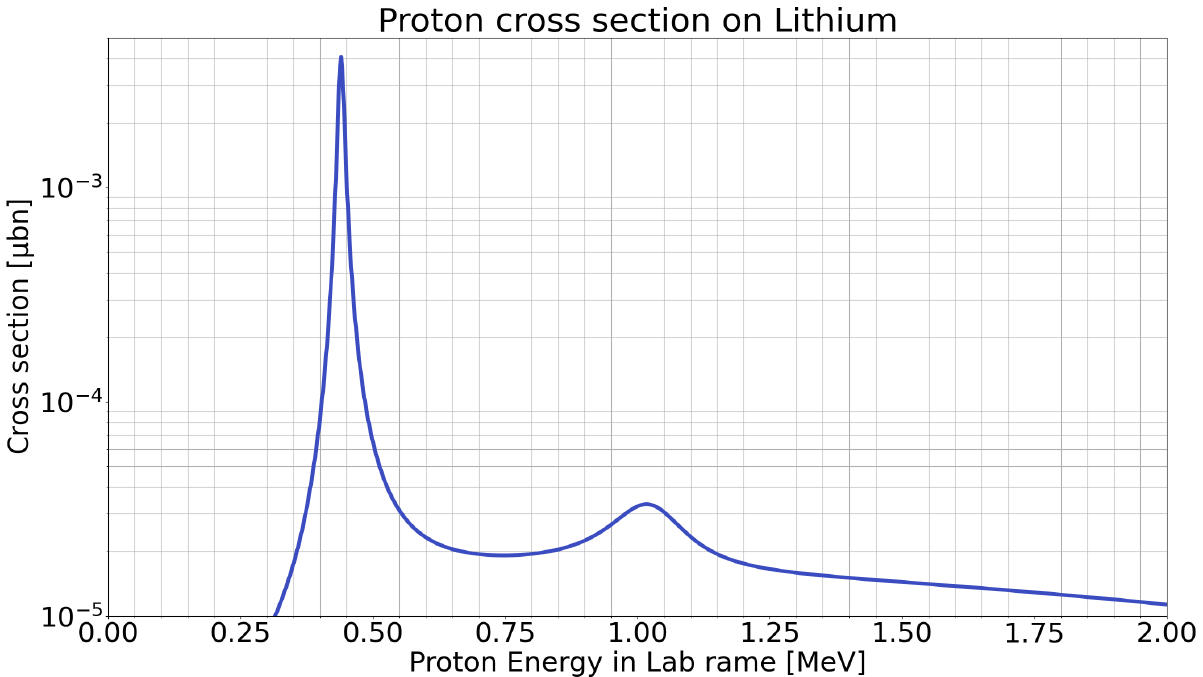
\includegraphics[width = 0.8\textwidth]{Figures/X17/pLi_crossection.png}
            \caption{Shape of the cross-section as a function of the proton energy \cite{X17:crossections} with two resonances.}
            \label{fig:X17:resonance}
        \end{figure}
        
        \begin{figure}
            \centering
            \subfloat[The first resonance occurs at a proton energy of $E_p=\SI{441}{keV}$, leading to a \SI{17.64}{MeV} excited state, while the second resonance, observed at $E_p=\SI{1030}{keV}$, results in the \SI{18.15}{MeV} state.]{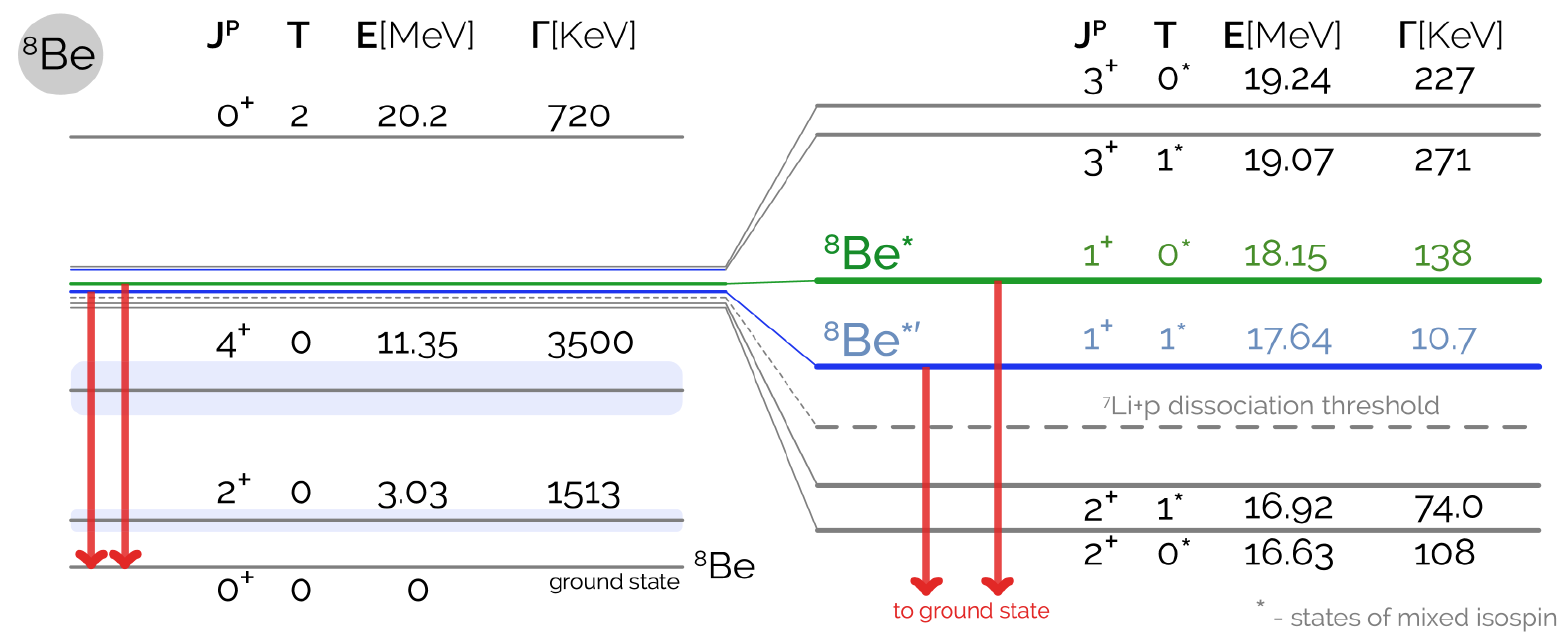
\includegraphics[height = 3.9cm]{Figures/X17/Be_levels.png}}\hfill
            \subfloat[Additionally to the ground level, both states can decay to the first excited level at $E=\SI{3.03}{MeV}$.]{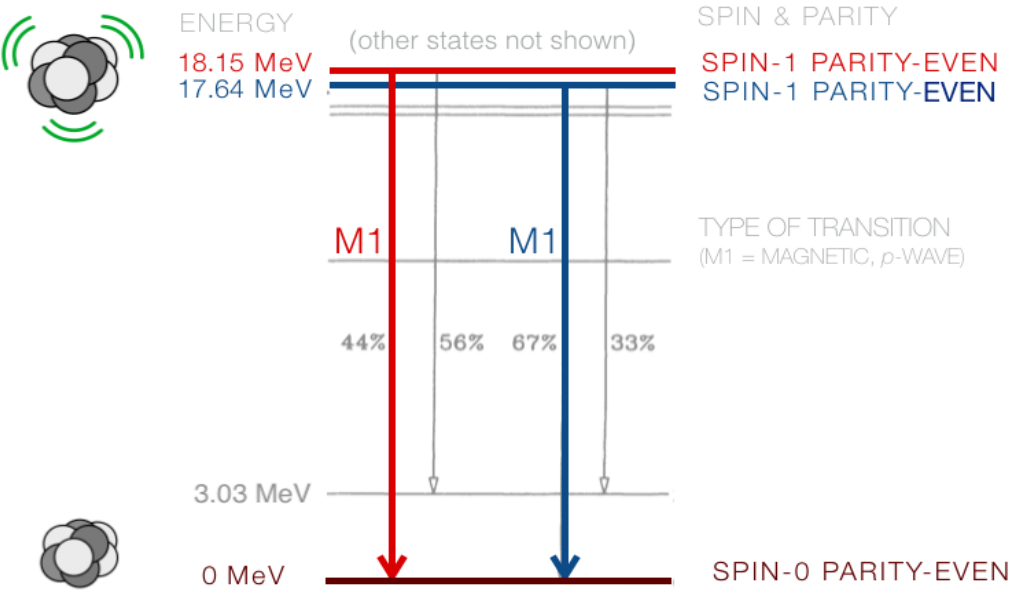
\includegraphics[height = 3.9cm]{Figures/X17/Be_levels_mixing.png}\label{fig:X17:states:b}}          
            \caption[Energy levels and transitions of \ce{^8Be}]{The proton-Lithium reaction exhibits two distinct resonances, shown in Fig.~\ref{fig:X17:resonance} \cite{X17:crossections} and different transitions \cite{X17:Elevels:2004}. The relative fractions of these processes are illustrated in Fig.~\ref{fig:X17:states:b}.}
            \label{fig:X17:states}
        \end{figure}

    \status{review}
    \subsection{The esults}
        What the ATOMKI collaboration found was an excess at $\sim\SI{140}{\deg}$ in the IPC. 
        The initial result yielded an invariant mass of $M = 16.70\pm0.51$~MeV \cite{X17:Anomaly:2015}, later refined to $M=16.94\pm0.12\pm0.20$~ MeV \cite{X17:2023}.
        These results were confirmed studying the \ce{^3H(p,\g)^4He} and \ce{^11B(p,\g)^12C}.\\
        After these results, Zhang and Miller \cite{X17:Zhang:2017}\cite{X17:Zhang:2020}\cite{X17:Zahng:2021} improved the reaction model to predict the cross sections. 
        Unfortunately, this model could not explain the excess.\\
        The latest entry was the preliminary result by the  University of Sciences in Hanoi \cite{X17:Hanoi:2023}.
        Unfortunately, all these studies have the same limitation: the measurements were done with a planar configuration,  on the plane perpendicular to the proton beam, as shown in Fig.~\ref{fig:X17:ATOMKI}.
        A study with wider acceptance is required \cite{X17:2023}, and this was what sparked the MEG II interest.

        \begin{figure}
            \centering
            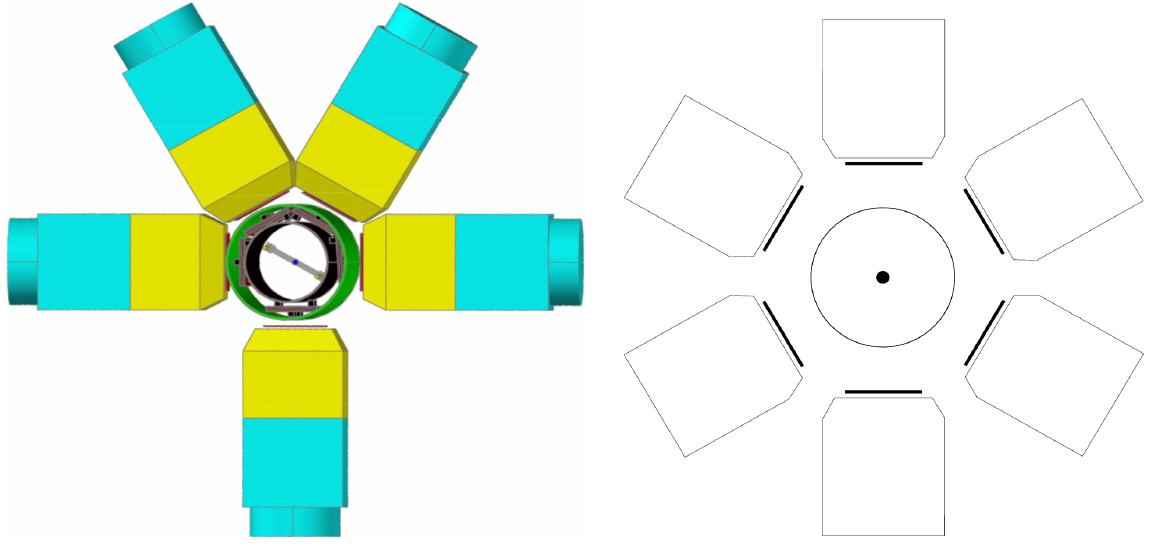
\includegraphics[width = 0.8\textwidth]{Figures/X17/Atomki_geometry.png}
            \caption{The planar geometry is the one chosen in all searches to date. In both versions, the energy is measured with plastic scintillators while the position is measured with a multi-wire proportional chamber, later upgraded to double-sided silicon strip detectors.}
            \label{fig:X17:ATOMKI}
        \end{figure}
        
\status{review}
\section{X17 in MEG II}
    After reading with great interest the papers from ATOMKI, the MEG collaboration started evaluating if repeating this measurement was achievable with the MEG II apparatus.
    In 2022 the first data collection was performed but the time constraints, required to keep the main focus of the experiment on $\upmu \rightarrow \upgamma e$, meant not all the necessary preparatory studies could be performed.
    The details of this first data-taking will be skipped and we will move directly to the second campaign, performed in 2023. 
    To be underlined is that this first campaign was cardinal in the rapid development of the tools required for the rest of the search: MC simulation, triggers, and analysis.
    Through the analysis of the data collected in 2023 some upgrades are ongoing and more data will be collected in 2024.
        
    \status{review}
    \subsection{Magnetic field choice}
        The first step is to identify the magnetic field required. 
        The geometry of the MEG II detector, in junction with the magnetic field, defines the acceptance of the produced particles.
        Given the nature of the COBRA magnet, the parameter here is the scaling of the magnetic field.
        Thorough simulations were run to optimize the scaling factor, finding the best compromise between the efficiency for signal and background reconstruction to be $B_{X17}=0.15\times B_{MEG}$. 
        This value can be roughly estimated considering that a scale factor of 1 is optimized for positrons of \SI{53}{MeV} while the pair produced by the X17 decay should be roughly at \SI{8}{MeV} ($8/53\approx 0.15$). 
        In reality, the hypothetical X17 would be produced with a boost, placing the energy of the pair particles in the range $[5.9,12.2]$~MeV.
        In 2022 and 2023 data were collected at 15\% 16\% and 17\% and the optimal value was found to be the first.
        This translates to an energy acceptance $[\sim7.5,\sim10.8]$~MeV.
        
    \status{review}
    \subsection{Target}
        The setup for the target has been optimized with dedicated studies \cite{X17:Meucci}. 
        The final design is quite straightforward: a carbon fiber vacuum chamber mounted at the tip of the insertion system of the CW bellows system; a mounting system, made of copper, holds different types of targets at \SI{45}{\deg}.
        The bellows system is the one used for XEC weekly calibrations and will be not discussed.
        
        \paragraph{Vacuum and mechanical structure}
        The thickness  (\SI{400}{\micro\meter}) and diameter (\SI{13}{cm}) of the carbon fiber vacuum chamber have been optimized via dedicated simulations for both integral structure and particle interaction.
        After receiving the carbon fiber, the chamber was glued to an aluminum flange and end-cap, with three stainless steel rods and three acrylic rings to reinforce the structure, and tested for vacuum.
        This setup is shown in Fig.~\ref{fig:X17:holder}.
        The mechanics of holding the target itself is also shown and it is made of copper.
        The reason for using this material is to improve the dissipation of the heat generated by the beam on the target.
        This, unfortunately, means a good percentage of the transition leading to a photon (meaning not an IPC) will generate an external pair (EPC) when the photon interacts with the copper.
        This contribution is bigger at lower angles, meaning IPC are the one dominating the region of interest.
        To reduce the contribution from EPC, the copper ring holding the target was later made thinner. 

        \begin{figure}
            \centering
            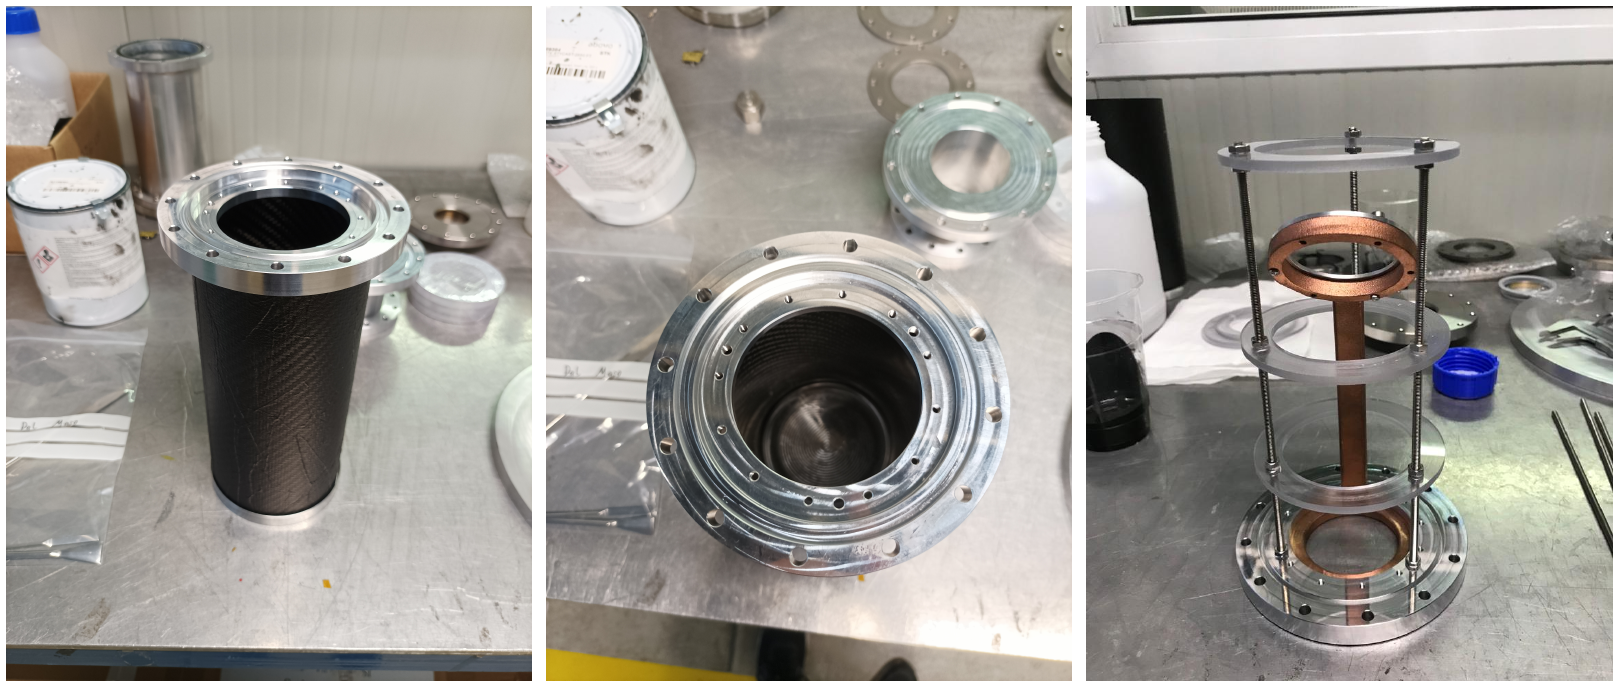
\includegraphics[width=\linewidth]{Figures/X17/X17_holder.png}
            \caption[X17: Vacuum chamber and target mechanics]{Construction of the carbon fiber vacuum chamber and picture of the copper arm used to hold the targets and of the internal structure of the chamber.}
            \label{fig:X17:holder}
        \end{figure}
        
        \paragraph{Lithium targets}
        The interesting process requires Lithium atoms but Lithium targets tend to be unstable. 
        Among the options studied, \ce{LiF} and \ce{Li_{3.6}PO_{3.4}N_{0.6}}\footnote{The fraction of the different atoms depends on the production process, which in this instance was \textit{sputtering}. These were the values measured for the target produced at PSI.} were the most promising, both on Cu substrate.
        \ce{LiF} targets were produced by INFN Legnaro while \ce{LiPON} targets were produced at PSI.
        Looking back we now know that the spattering process behind the production of the \ce{LiPON} targets resulted in a poorly characterized end-product (more on this in a following section). 
        Some data were acquired using the \ce{LiF} target, but the Fluorine has resonances \ce{^17F(p,\alpha\gamma)^16O} at \SI{6.13}{MeV}, \SI{6.92}{MeV}, and \SI{7.12}{MeV} with a cross-section much higher than the one of the Lithium \cite{}.
        This meant that the events of interest were hidden by the F resonance.
        For this reason, the collaboration opted for LiPON.
        Some spectra taken with the BGO for both targets are in Fig.~\ref{fig:X17:BGO:targets}.

        \begin{figure}
            \centering
            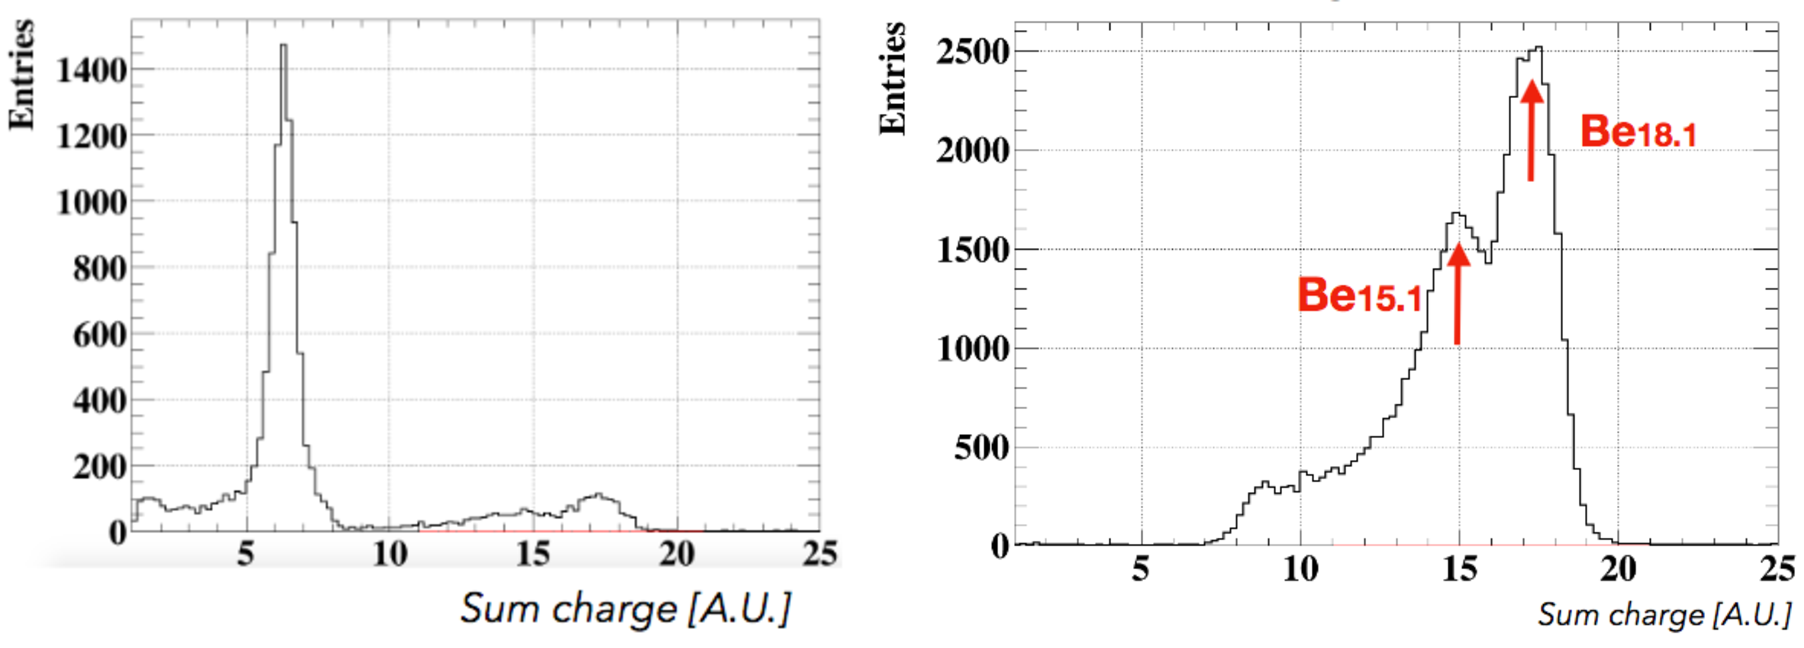
\includegraphics[width=0.9\linewidth]{Figures//X17//X17_Feb2023/X17_BGO_targets.pdf}
            \caption[X17:BGO LiF and LIPON]{BGO spectrum for E$_p$ = 500 keV with LiF target (left) and  for E$_p$ = 1080 keV LIPON target (right).}
            \label{fig:X17:BGO:targets}
            \end{figure}
            
    \status{review}
    \subsection{MC simulations}
        To develop a complete simulation, the obvious decision was to implement the details in the pre-existing MEG II simulation.
        This is \textit{GEM}, based on \gf, which returns the detector responses to the physics event. 
        After that, the \textit{bartender} converts the simulation into realistic waveforms, to be analyzed with the standard MEG II hit reconstructions.
        The track-finding algorithms and trigger strategies can be then tested on realistic events.
        The core aspects of the simulation are:
        \begin{outline}
            \1 The \SI{15}{MeV} line is simulate with \SI{3}{MeV} width, while the \SI{18.1}{MeV} is monochromatic
            \1 The excited beryllium is at rest
            \1 Isotropical decay in the rest frame of the X17 ($M=\SI{16.7}{MeV/c^2}$)
        \end{outline}     
        While IPC and X17 can be easily generated, EPC are more challenging because the particle generated is the $\g$ which then converts.
        The aim for the MC statistics is to produce: \SI{2e5}{X17}, \SI{e6}{IPC18}, \SI{e6}{IPC15}, and \num{e9} $\g$ to generate EPC.
        In the following, the MC data will be the one produced in July 2023.

        \paragraph{IPC}
        IPC events at 18 MeV and 15 MeV are simulated in the following steps: Proton energy loss follows a Gaussian distribution, with mean and standard deviation determined from GEANT4 simulations; 
        the interaction depth of the proton is generated based on the randomly obtained energy loss;
        the IPC spectrum is generated using the Zhang-Miller cross-section, which includes non-resonant proton direct capture;
        the transition energies are generated separately. Zhang-Miller model, originally for the 18.15 MeV transition, is also applied to the 15.12 MeV transition, introducing additional uncertainty. The cross-section parameters are determined using old photon data and may benefit from updated measurements.
    
    \status{review}
    \subsection{Data acquisition(s)}
    \label{sec:X17:beamtuning}
        We went through different data-taking periods. 
        The first was at the end of 2022 and lasted 3 weeks while the second was in Feb. 2023 and lasted 4 weeks.
        During the first period, we collected data used to develop the MC simulations, event reconstruction, and optimize the trigger.
        At this stage, the understanding was only partial but we deemed it sufficient to collect useful data as an intermediate step.
        The second period was the main data acquisition. 
        A short data-taking in May 2023 followed to collect some photon spectra with the XEC.
        Additional studies were performed in Nov. 2023 and Feb. 2024.
        These last two will be discussed later.

        \paragraph{Setup} Although this search is done with the MEG II apparatus, some minor changes should be underlined.
        The X17 data were collected while the MEG II acquisition was not ongoing. This means it was in parallel with the maintenance of the XEC, which was undergoing annealing to recover MPPC PDE.
        For this reason, we relied on two auxiliary detectors, shown in Fig.~\ref{fig:X17:Brillance}: the BGO and an additional 3-inch Lanthanium Bromide crystal (\ce{LaBr3} `Brillance'), both read by PMTs.
        We also took data with the BGO in different positions to study the asymmetry of the spectra.

        \begin{figure}
            \centering
            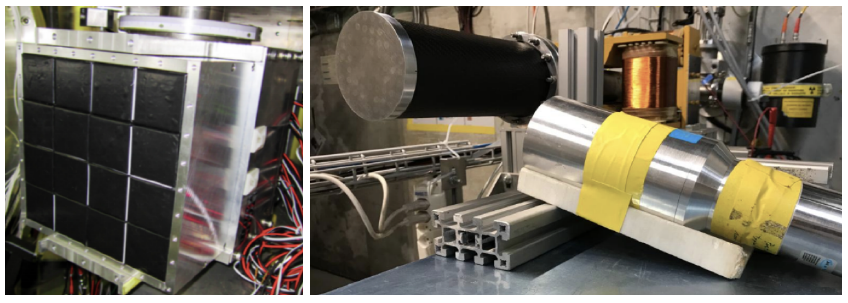
\includegraphics[width = 0.9\textwidth]{Figures/X17/BGOandBrillance.png}
            \caption[X17: Auxiliarly detecotrs]{Pictures of the auxiliary detectors: BGO, on the left, and Brillance, on the right.}
            \label{fig:X17:Brillance}
        \end{figure}
        
        \paragraph{Beam tuning}
        The beam tuning was performed by substituting the end cap of the proton beam line with a transparent cap with a quartz crystal. 
        The proton beam produces visible photons hitting the crystal so the beam position can be observed.
        Normally this operation would be done while the upstream side of COBRA is not closed, allowing the installation of a webcam that gives instant feedback on the beam position.
        This was not the case so we were forced to use the camera installed inside COBRA for MEG II target monitoring.
        This camera has some settings for \textit{gain} and \textit{aperture} but is controlled using a script in \textit{ssh} and to view the picture first is necessary to move them locally, making the whole procedure somewhat cumbersome.
        Key aspects of the tuning:
        \begin{outline}
            \1 Energy: This parameter is controlled by the \textit{Terminal Voltage} of the CW. 
            \1 Position: This parameter is controlled by the three dipoles of the CW beamline. The change of the position for different values of the dipoles at \SI{500}{keV} is shown in Fig.~\ref{fig:position_500keV}.
            \1 Focus: This parameter is controlled by the \textit{Extraction Voltage} of the CW. Fig.~\ref{fig:focus_500keV} shows how the beam spot changes as a function of this parameter.
        \end{outline}

        \begin{figure}
            \centering
            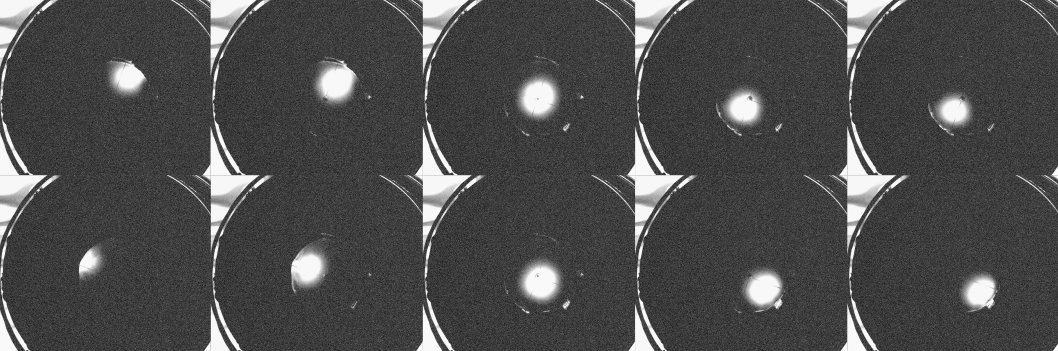
\includegraphics[width = \textwidth]{Figures/X17/beamtuning/psotion_500keV.png}
            \caption{Position of the proton beam at \SI{500}{keV} when changing the current in the dipoles (the vertical dipole V and only one of the two horizontal dipoles H). In the first row, H is changing and the beam moves diagonally. In the second row, V moves the beam on the perpendicular diagonal.}
            \label{fig:position_500keV}
        \end{figure}
        \begin{figure}
            \centering
            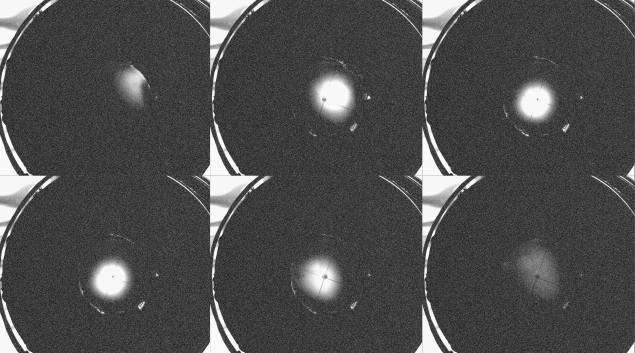
\includegraphics[width = \textwidth]{Figures/X17/beamtuning/focus_500keV.png}
            \caption{Focus of the proton beam at \SI{500}{keV} when changing the \textit{extraction voltage} of the CW: values in the range $6\divisionsymbol15$ keV. Is clearly visible for extreme values the beam barely reaches the crystal.}
            \label{fig:focus_500keV}
        \end{figure}
        \noindent
        After a careful scan, working points at different energies were chosen: the most relevant are the ones for \SI{500}{keV} and \SI{1080}{keV}.
        It is of interest to notice that \SI{1080}{keV} is the balance between what was previously discussed and the limitations of the CW machine: a higher ($\sim$\SI{1100}{keV}) energy would be a better choice but the nominal upper limit of the machine is \SI{1}{MeV}, meaning having it running stably at \SI{1080}{keV} is already an achievement.
        To the best of our knowledge, the beam at COBRA center during data-taking was $(x, y) = \SIlist{2; -2}{mm}$; $(\sigma_x, \sigma_y) = \SIlist{2; 2}{mm}$.\\

        \noindent
        After the first tuning, these parameters were used for the different data-takings. 
        In Sec.~\ref{sec:X17:H2+} we will see why this beam-tuning had a fundamental flaw, linked to the presence of \ce{H2^+}.

        \paragraph{Trigger and Rates}
        The X17 trigger developed requires 18 hits on both CDCH ends\footnote{Unfortunately, at trigger level we cannot match the same wire on both sides} and at least one hit in the pTC. 
        At the same time, BGO, Brillance, pTC single, CDHC Track, and pedestal trigger were acquired, with a prescale factor. 
        A comparison between the trigger rate in data and MC has been made for a proton current of 6$\mu$A. 
        At this current, X17 trigger rate is about 30 Hz on data.
        Based on measured gamma rates on BGO (60 kHz), trigger efficiencies estimated from simulation (0.039$\%$ and 6.5$\%$ for EPC and IPC respectively), and the IPC BR (0.0032), the background rates can be estimated. 
        It is found that expected trigger rates are 23 Hz and 12 Hz for EPC and IPC respectively, for a total rate of about 35 Hz, in fair agreement with the measured 30 Hz at \SI{6}{\micro\ampere}.
        
\status{review}
\section{Data analysis}
    My contribution to the data analysis was only partial so I will not go into much detail. 
    Even so, at least a broad overview of the analysis status at the time of writing is in order.
    Most of the studies on event reconstruction and quality cuts were performed by Hicham Benmansour, while the Likelihood analysis was developed by Giovanni Dal Maso \cite{Giovanni}. 
    I contributed in different aspects but mainly during the development of the Likelihood analysis and BGO analysis.

    \status{review}
    \subsection{Pair reconstruction}
        The first step for this search is to correlate particles and create $\e \Ae$ pairs. 
        This is not a given in an experiment that was developed for a different task, namely reconstructing $\e$ and $\g$. 
        The idea was, of course, to adapt the existing reconstruction code to the new aim.
        
        \paragraph{\textbf{B} inversion}
        As well known, particles of opposite charge behave symmetrically in the same B field.
        This means the $\e$ reconstruction in $\textbf{B}=B\hat{z}$ is equivalent to reconstructing a $\Ae$ in $\textbf{B}=-B\hat{z}$.
        This is a simple change to apply to the reconstruction code but holds only in the assumption the two particles behave in the same way while interacting with the different parts of the experiment.

        \paragraph{Track selection}
        A series of quality selections is applied to single tracks. 
        The purpose is to reject tracks that are reconstructed with the incorrect sign. 
        These tracks, called \textit{fake}, are often short or have low hit density and are often close to COBRA center at $z=0$.
        Fig.~\ref{fig:X17:tracks}
        shows the requirements for the number and quality of hits while Fig.~\ref{fig:X17:fakes} shows the effectiveness of the final selection in reducing the fake pairs to a more simple selection in X17 data (E$_{sum}$ side-band region, as defined in ~\ref{sec:blind}).
        The requirements are:

        \begin{itemize}
            \item successful propagation of the track to the beam axis;
            \item at least 10 good hits (ngoodhits) on track;
            \item if 11 $\leq$ ngoodhits $\leq$ 16, track hit density should be $>$ 1.1 hits/cm;   
            \item $|z_{vertex}-z_{beamspot}|$ $<$ 2.5 cm, $z_{vertex}$ being the z coordinate of the point of closest approach to the beamline and $z_{beamspot}$ the best estimate of the z coordinate of the beam spot on target;
            \item  time order in the hits $T_{0,lasthit}>T_{0,firshit}$;
            \item  $(z_{lasthit}-z_{firshit}) \times z_{firshit} > 0$, to ensure the track goes away from the target;
            \item distance 1$^{st}$ hit to vertex smaller than 35 cm, to ensure the first turn is not missed;
            \item half-turn tracks (tracks which never exit the chamber) should have a hit density $>$ 0.8 hits/cm and a track score $>$ 20, track score being defined as $\mbox{ngoodhits} + 10 \times \mbox{track hit density}$;
            \item  $|z_{firsthit}|>2.5$ cm;
            \item no hits with opposite $z_{hit}$;
            \item each half-turn should have a standard deviation for the consecutive hits distance below 0.9 cm (to ensure most hits are included in the track fit);
            \item $|z_{mean}|>2.0$ cm, $z_{mean}$ being the average of $z_{hit}$ for all good hits (to ensure the track is far enough from the target);
            \item $z_{mean} \times (\theta - 90^o) < 0$.
        \end{itemize}

        \paragraph{Pair selections}
        For events where at least one positron track and at least one electron track pass the previous selection, pair selection criteria are applied:
        \begin{itemize}
            \item the $\e$/$\Ae$ tracks should have no hits in common, to ensure no track is reconstructed with the wrong sign-
            \item the distance between the vertices of both tracks should be $\leq$ 3 cm.
        \end{itemize}


        \begin{figure}[]
            \centering
            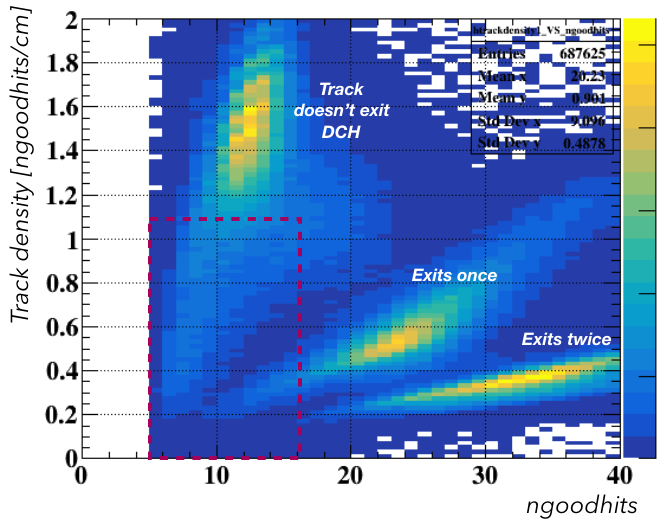
\includegraphics[width=0.8\textwidth]{Figures/X17/Analysis/halfturn_cond.png}
            \caption{Track density vs ngoodhits. Three types of tracks can be observed with increasing ngoodhits and decreasing density, tracks not exiting the chamber, tracks exiting it once and tracks exiting twice. The poorest quality tracks, in the red dashed rectangle, are rejected.}
            \label{fig:X17:tracks}
        \end{figure}

        \begin{figure}[]
            \centering
            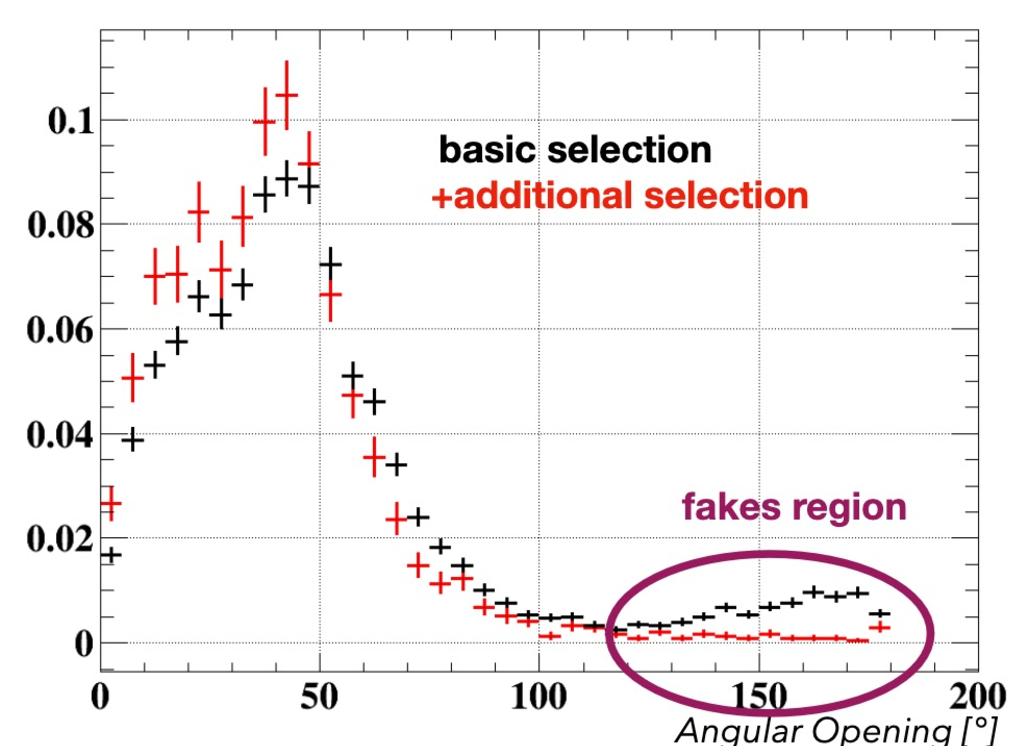
\includegraphics[width=0.8\textwidth]{Figures/X17/Analysis/Fake.pdf}
            \caption{E$_{sum}$ distributions for the X17 data (E$_{sum}$ sideband region, as defined in ~\ref{sec:blind}) before (black dots) and after (red dots) the cuts specific for removing fake pairs, described in the text.}
            \label{fig:X17:fakes}
        \end{figure}

        \paragraph{Track and pair efficiencies}
        When considering the whole reconstruction, the efficiency for the different types of events is summarized in Table~\ref{tab:X17:efficiency} and Fig.~\ref{fig:X17:totaleff} shows the total efficiency on X17 events (trigger, acceptance, and reconstruction efficiency) as a function of the angle of the reconstructed X17 momentum direction to the beam axis.
        
        \begin{table*}[]
            \centering
            \begin{tabular}{|c|c|c|c|c|c|c|}
                 \hline
            &  signal & IPC        & IPC         & EPC      & EPC      & data   \\
            &   & 18 MeV        & 15 MeV         & 18 MeV      & 15 MeV   &    \\
             \hline
                 trigger selection  & 14\% & 4.5\%& 3.9\%&  0.032\% & 0.027\% &  100\%   \\      \hline
                  positron track selection (wrt trg)    & 38\%    & 37\%& 33\%&  27\%& 21\%& 8\%    \\      \hline
                        pair selection (wrt trg)          & 9\% & 8\%& 5\%&  5\% & \textcolor{red}{0.4\%}&   1.4\%  \\      \hline
                \end{tabular}
            \caption{Efficiency of the different reconstructions.}
            \label{tab:X17:efficiency}
        \end{table*}

        \begin{figure}[]
            \centering
            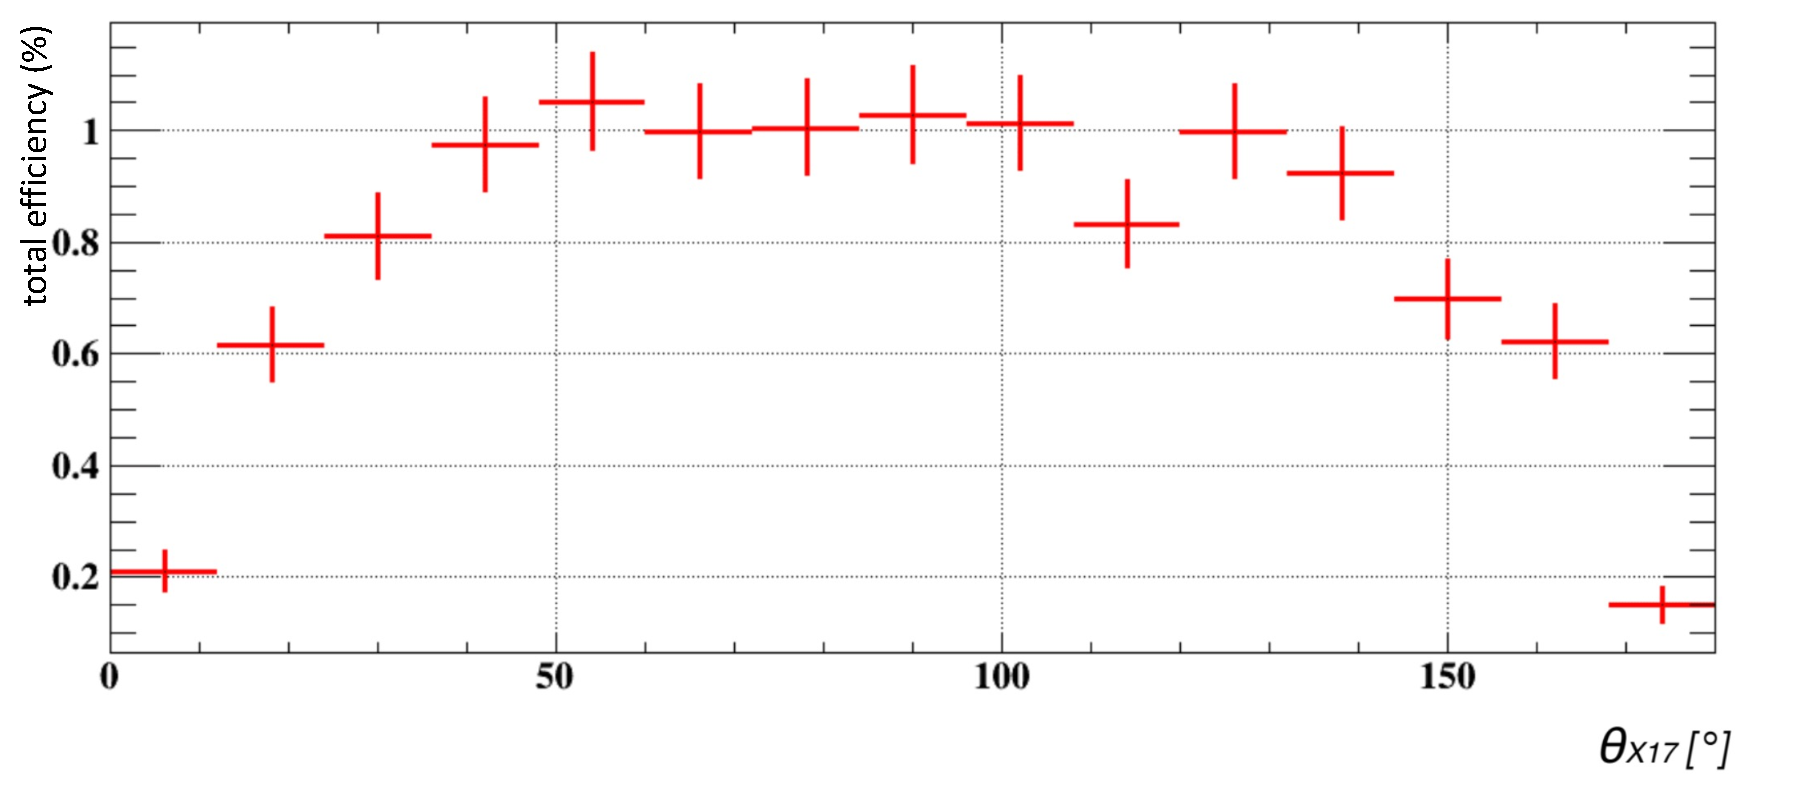
\includegraphics[width=0.8\textwidth]{Figures/X17/Analysis/TotalEff.pdf}
            \caption{Total efficiency on X17 events (trigger, acceptance, and reconstruction efficiency) as a function of the angle of the reconstructed X17 momentum direction to the beam axis.}
            \label{fig:X17:totaleff}
        \end{figure}

        \status{review}
        \subsection{Angular corrections}
        Due to multiple scattering in the air between the target and CDCH, some tracks are reconstructed far ($\sim$cm) from the true vertex, this can be improved by studying the correlation between the reconstructed vertex position and the reconstructed momentum direction. 
        Fig.~\ref{fig:X17:corrtheta} and ~\ref{fig:X17:corrphi} show the correlation between the residuals of the polar and azimuthal angle, as a function the residuals on the x, y, z coordinates, on MC. 
        A strong correlation can be observed (and linearly correct) in the residuals of the polar angle vs the residuals of the z coordinate, as well as in the residual of the azimuthal angle vs the residuals of the x coordinate.  
        The true value of x and z can be approximated to be zero.
        Fig.~\ref{fig:corrIPC} and \ref{fig:corrX17} show the effect of the correction in the opening angle and invariant mass resolutions for IPC18 and X17 MC events.
        
        \begin{sidewaysfigure}[]
            \centering
            \subfloat[Residuals of the polar angle as a function of the residuals of the x, y, z coordinates, on MC.]{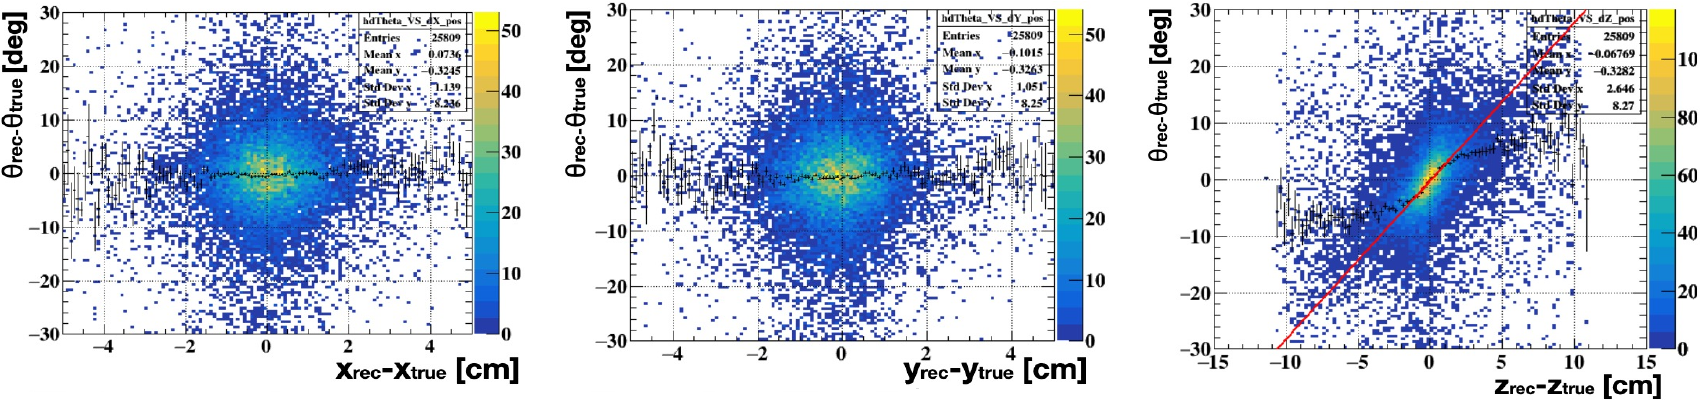
\includegraphics[width=0.9\textwidth]{Figures/X17/Analysis/CorrTheta.png}\label{fig:X17:corrtheta}}\\\vspace{1cm}
            \subfloat[Residuals of the azimuthal angle as a function of the residuals of the x, y, z coordinates, on MC.]{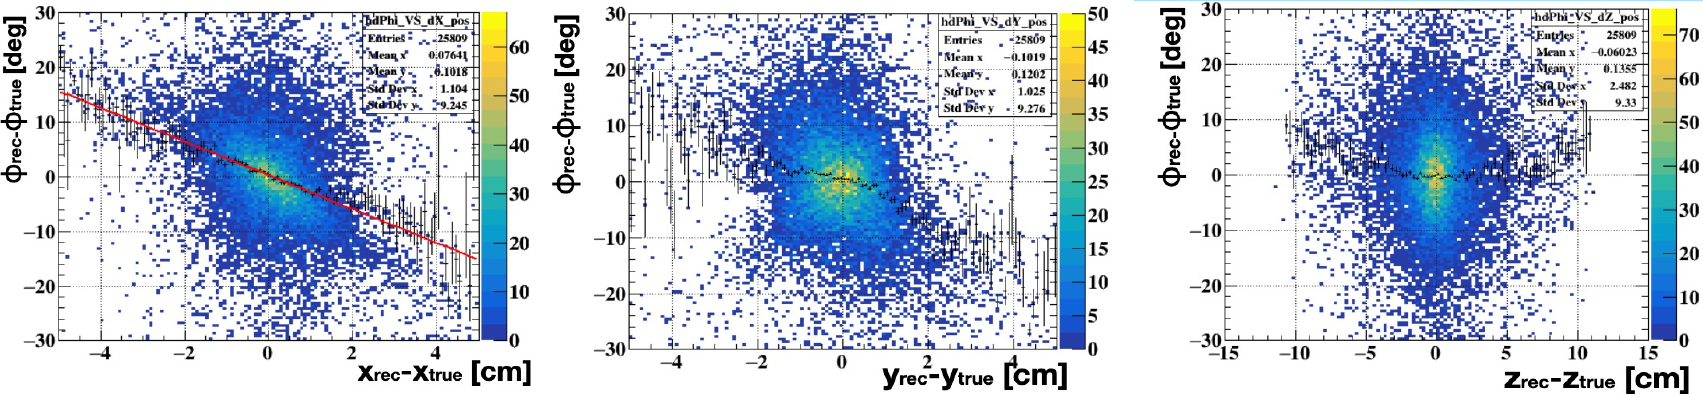
\includegraphics[width=0.9\textwidth]{Figures/X17/Analysis/CorrPhi.png}\label{fig:X17:corrphi}}
            \caption[X17: Angular correlations]{The correlation of vertex displacement and momentum direction are modeled and corrected.}
        \end{sidewaysfigure}
        


        \begin{figure}[]
            \centering
            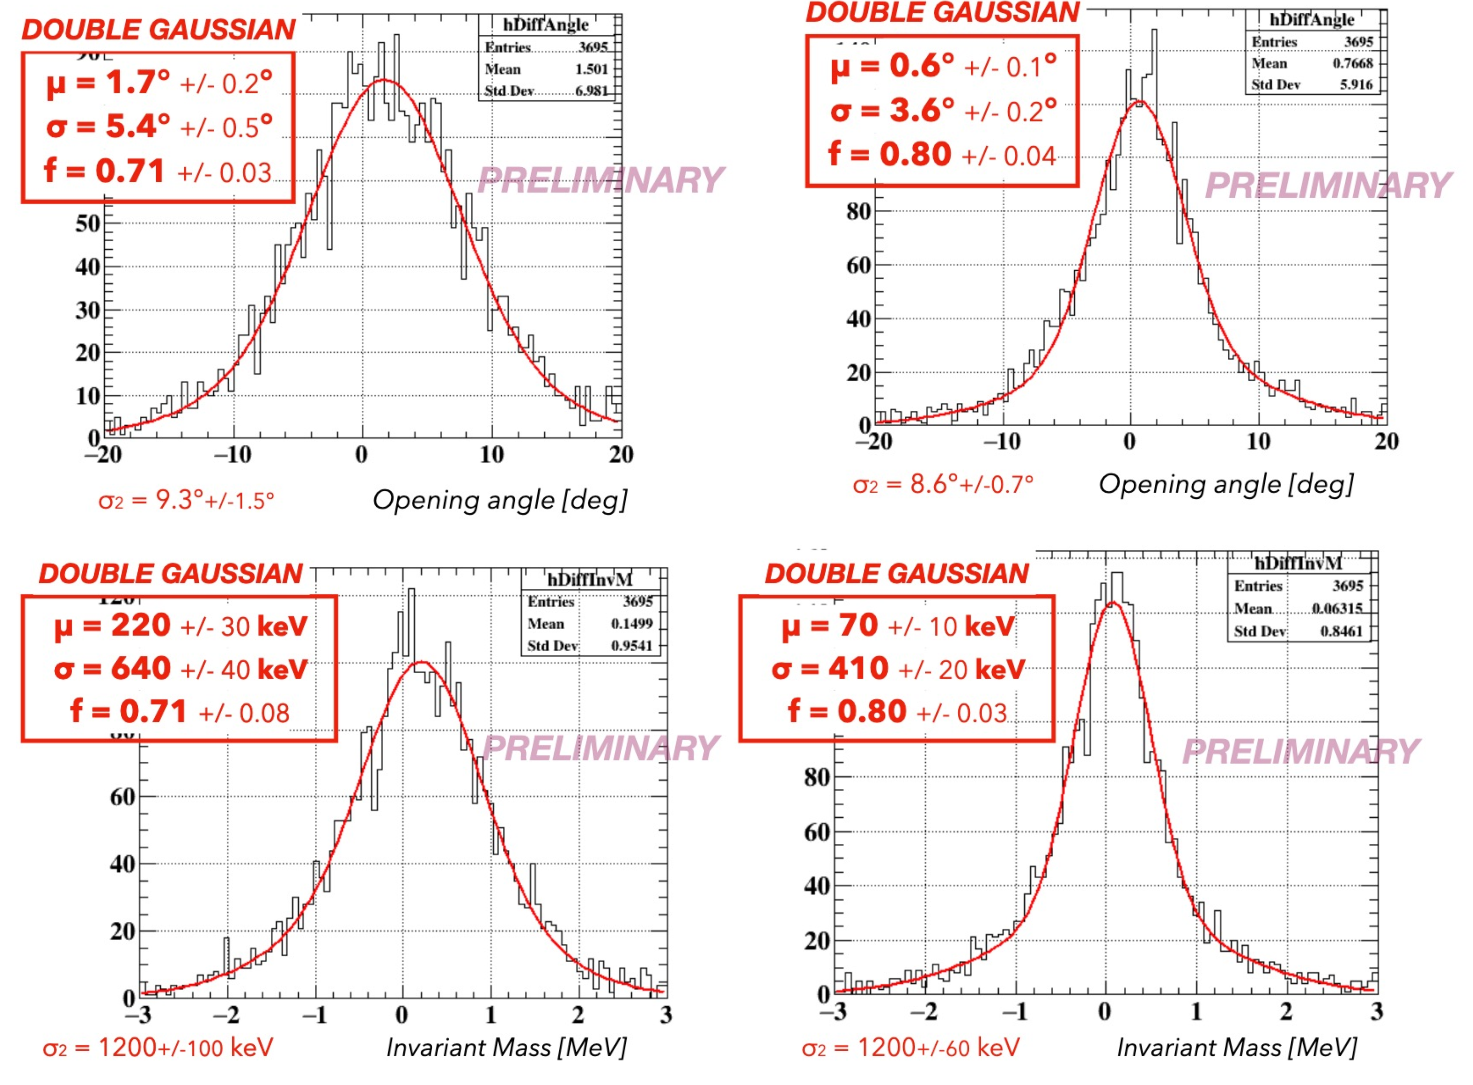
\includegraphics[scale=0.5]{Figures/X17/Analysis/AngCorrReso.pdf}
            \caption{Opening angle resolution (upper plots) and invariant mass resolution (lower plots) for MC IPC18 events, fitted to a double Gaussian. On the left there is the distribution obtained without the angle correction, on the right the one with the angle correction.}
              \label{fig:corrIPC}
        \end{figure}
        %
        \begin{figure}[]
            \centering
            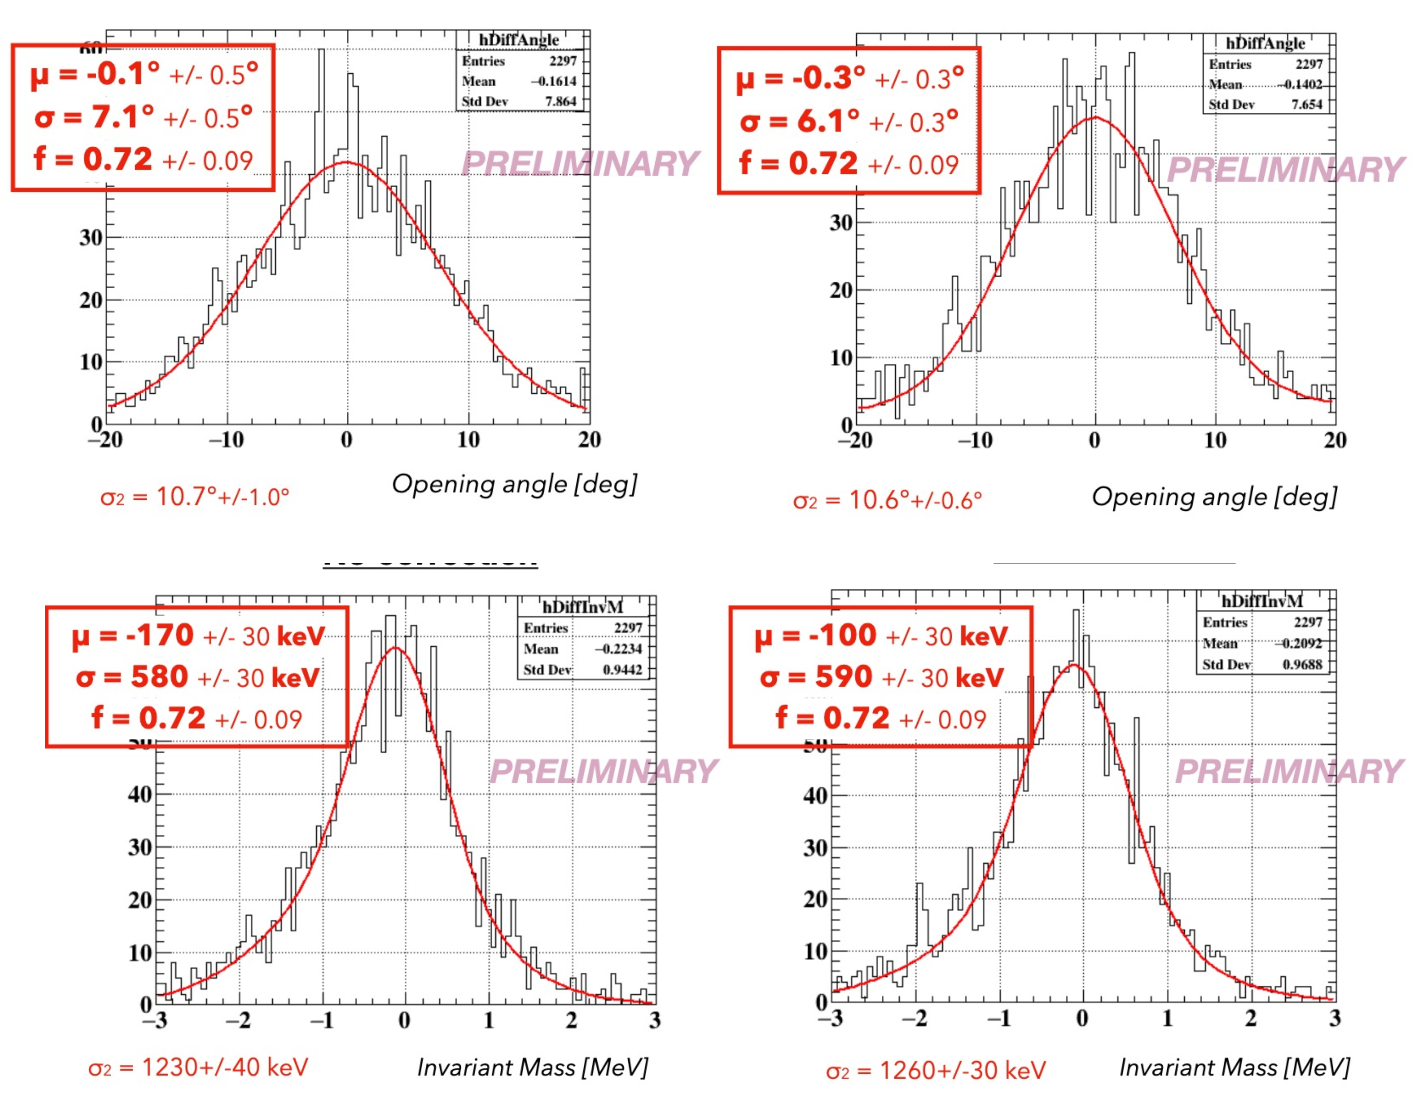
\includegraphics[scale=0.5]{Figures/X17/Analysis/CorrAngleX17.pdf}
            \caption{Opening angle resolution (upper plots) and invariant mass resolution (lower plots) for MC X17 events, fitted to a double Gaussian. On the left there is the distribution obtained without the angle correction, on the right the one with the angle correction.}
            \label{fig:corrX17}
        \end{figure}

        \status{review}
        \subsection{Vertexing}
        To improve the $E_{sum}$ and $\theta_{rel}$ resolution, a vertex fit has been introduced using the positron and electron state vertex at the z-axis POCA and the beam spot information.
        The procedure is:
        \begin{itemize}
            \item all tracks are fitted separately to the z axis POCA
            \item the best positron and electron tracks are selected
            \item the common vertex is searched with a beam spot constraint using the tool RAVE (Reconstruction in Abstract Versatile Environments), supported in GENFIT \cite{RAVE}\cite{GENFIT}. The beam spot constraint is defined as (x,y,z) coordinates plus the invariant matrix with $\sigma =\SI{3}{mm}$. 
        \end{itemize}
        Fig.~\ref{fig:vertexing} shows the comparison in the opening angle resolution for IPC18 and X17 MC with and without vertexing, obtaining a 25$\%$ improvement in the core resolution of a double Gaussian.
        
        \begin{figure}[htbp]
            \centering
            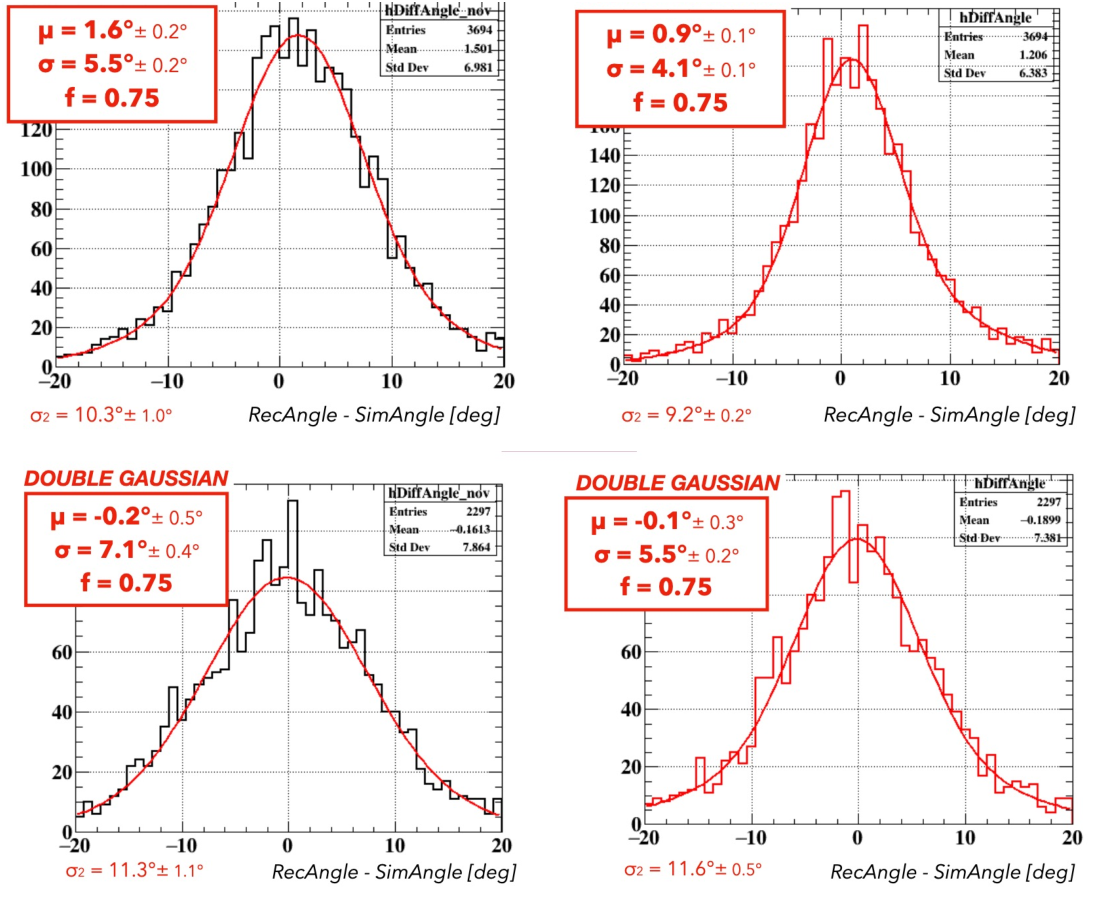
\includegraphics[scale=0.5]{Figures/X17/Analysis/Vertexing.pdf}
            \caption{Opening angle resolution for IPC18 (upper plots) and X17 (lower plots) MC, fitted to a double Gaussian. On the left, the distribution obtained without vertexing, and on the right the one with vertexing.}
             \label{fig:vertexing}
        \end{figure}

        \status{review}
        \subsection{Beam spot}
        Fig.~\ref{fig:beamspot1} shows the distributions of the reconstructed vertex at the target for positrons and electrons, on X17 data. 
        It can be noted that the vertices are off-center by 7 mm and the positron and electron vertices distributions are shifted versus one another.
        On MC, IPC vertices are correctly reconstructed (within 1 mm) while EPC vertices are reconstructed with a systematic shift toward negative y (most likely from the gamma anisotropy and a bias from the trigger) and there is a shift between positrons and electrons.
        The beam spot position on data has been determined according to the following procedure: the x coordinate was extracted from an IPC-enriched data sample at a low opening angle; the y coordinate was determined by fitting the data y distribution to the MC distribution where a 60$\%$-40$\%$ proportion has been assumed for EPC/IPC. The fit is shown in Fig.~\ref{fig:beamspotfit}.
        The values obtained are $(x, y) = \SIlist{-2; -3}{mm}$; $\sigma_x= \sigma_y = \SI{3}{mm}$.

        \begin{figure}[]
            \centering
            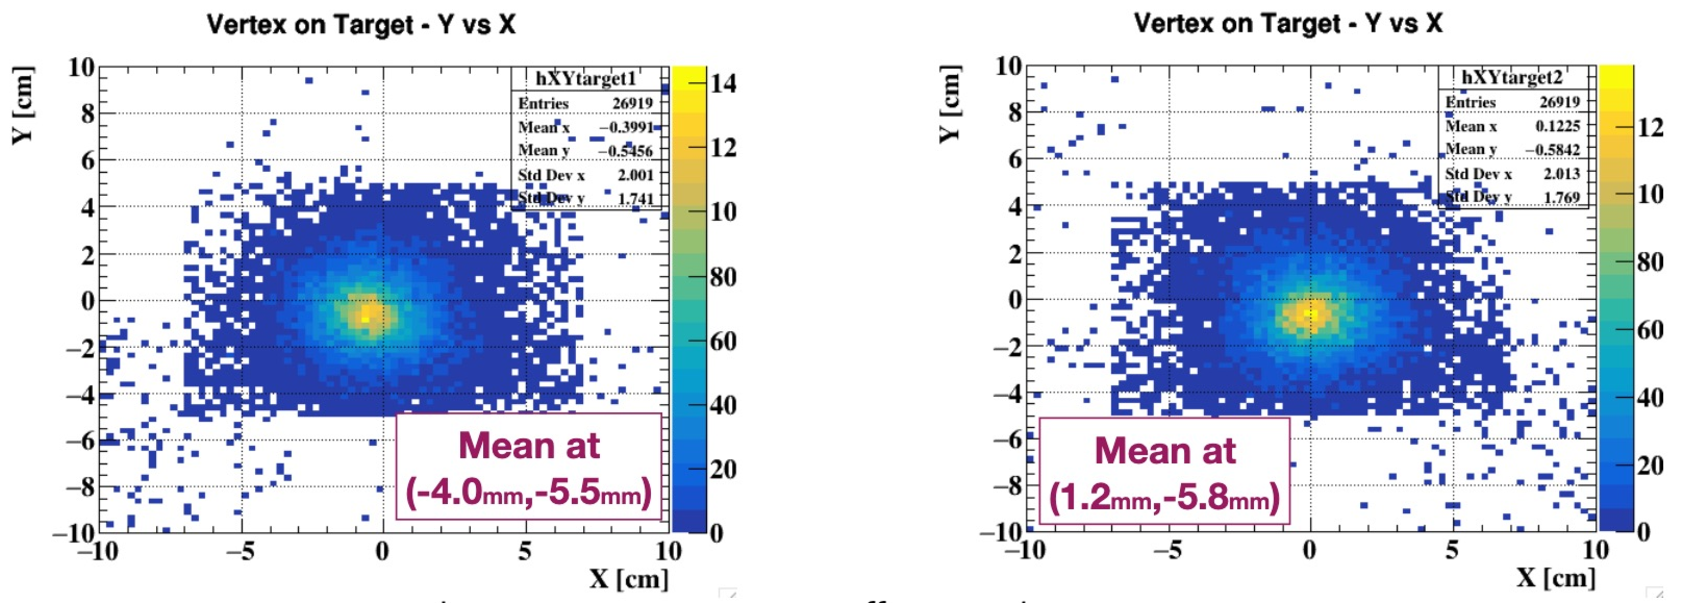
\includegraphics[scale=0.5]{Figures/X17/Analysis/BeamSpotData.pdf}
            \caption{Distribution of the reconstructed vertex position positrons (left) and electrons (right) on X17 data.}
             \label{fig:beamspot1}
        \end{figure}
        
        \begin{figure}[]
            \centering
            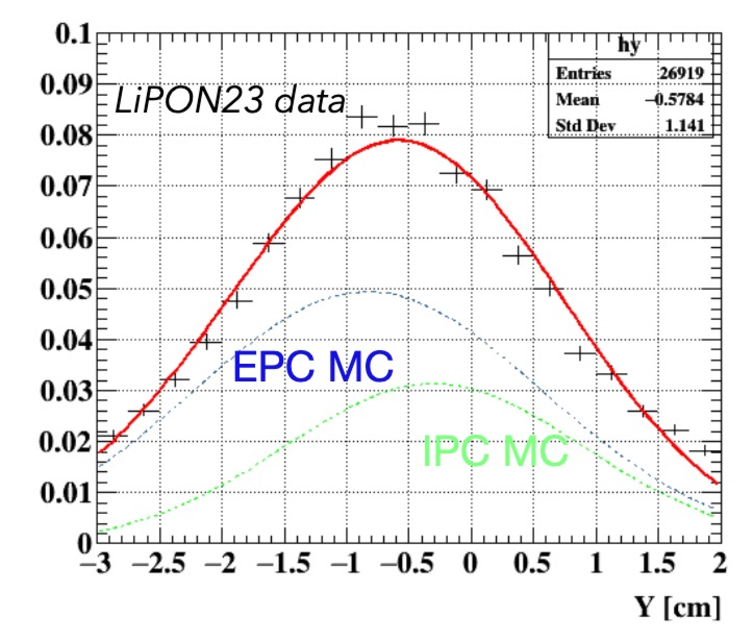
\includegraphics[scale=0.5]{Figures/X17/Analysis/BeamSpotFit.pdf}
            \caption{Y vertex distribution fitted to the MC: a 60$\%$-40$\%$ proportion has been assumed for EPC/IPC.}
            \label{fig:beamspotfit}
        \end{figure}

    \status{review}
    \subsection{Blinding strategy}\label{sec:blind}
    A blinded signal region has been defined according to the following conditions: $E_{sum}\in[\SI{16}{MeV},\ \SI{20}{MeV}]$ and $\theta_{rel}\in[\SI{115}{\deg},\ \SI{160}{\deg}]$.
    Fig.~\ref{fig:regions} shows, in the E$_{sum}$ vs $\theta_{rel}$ plane, the blinded signal region together with the relative angle sideband (16 MeV $<$ E$_{sum}$ $<$ 20 MeV and 0$^o$ $<$ $\theta_{rel}$ $<$ 115$^o$) and the E$_{sum}$ sideband (14 MeV $<$ E$_{sum}$ $<$ 16 MeV and 0$^o$ $<$ $\theta_{rel}$ $<$ 180$^o$).
    \begin{figure}[htbp]
        \centering
        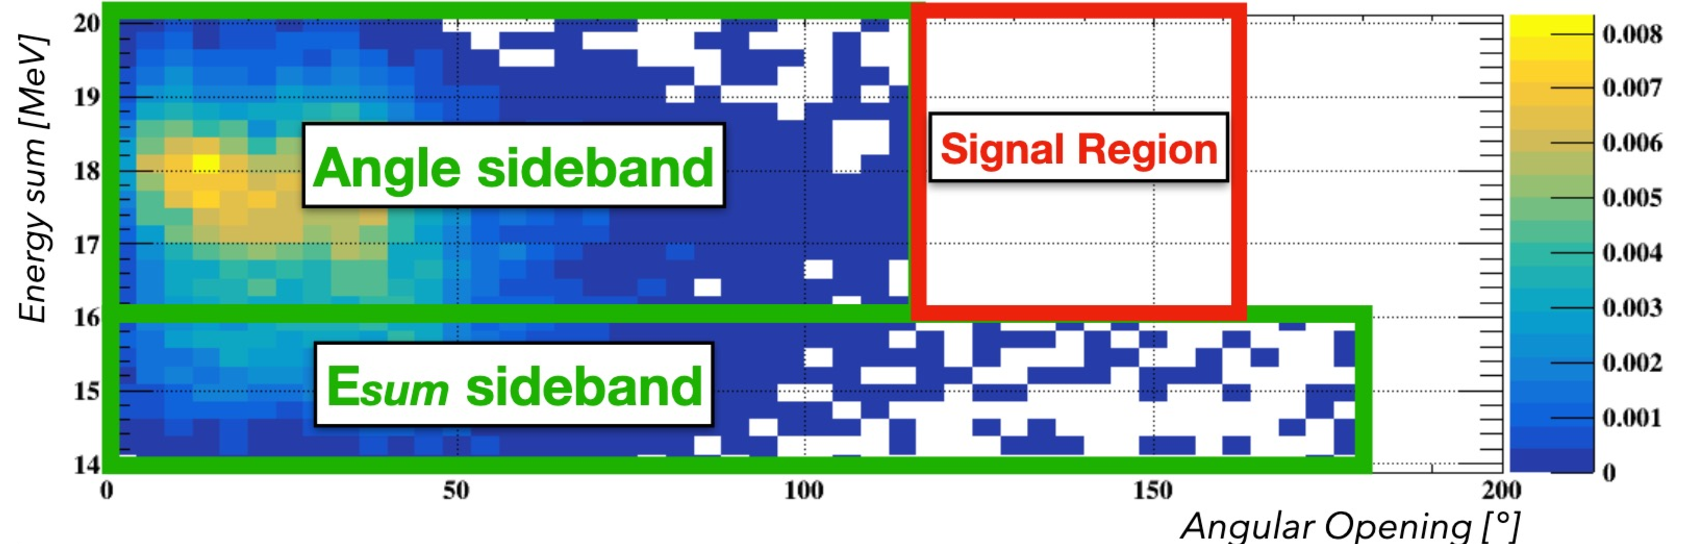
\includegraphics[width = 0.9\textwidth]{Figures/X17/Analysis/Regions.pdf}  
        \caption{Blinded signal region and sidebands in the E$_{sum}$ vs $\theta_{rel}$ plane.}
         \label{fig:regions}
    \end{figure}

    \status{review}
    \subsection{Likelihood analysis}
    \label{sec:X17:likelihood}
        Although the Feldman-Cousin approach is well-established in particle physics research, this was our first hands-on experience. 
        After studying the relevant papers \cite{feldman:1998}\cite{feldman:2011} and the internal notes of the collaboration, we decided to first develop a mock-up\footnote{The full description of the code will be here skipped but it can be found in the following         \href{https://github.com/gdalmaso96/X17_LL_mock_up}{\underline{git repository \faGithubSquare}}} to understand the framework necessary for a Feldman Cousin approach to data analysis.  
        The full-blown X17 analysis will be performed with the code already written for the MEG II analysis. 
        This code was developed and improved upon over many years and was both more robust and flexible. 
        Although I followed the whole procedure, the finalization of the mock-up and the transition to the MEG II code was done by Giovanni Dal Maso. 
        The broad idea is to extract the Probability Density Functions (PDF) parametrizing the spectra generated in GEM and benchmarked with the side-bends.
        This approach relies on the statistics of the MC production, which is unfortunately limited.
        An alternative method would be to implement background PDFs as histogram templates, as in the Beeston-Barlow \cite{X17:likelihood:BB}.
        All the missing details can be found in the PhD thesis of Giovanni Dal Maso \cite{Giovanni}.

        \paragraph{Likelihood}
        The likelihood is defined by five populations: X17, IPC15, IPC18, EPC15, and EPC18.
        Given the flexibility of the framework, the analysis can be 1D, in \textit{invariant mass/ relative angle} or 2D, adding the \textit{energy sum} and can be binned or un-binned.
        The likelihood is shown in Eq.~\ref{eq:X17:L}, in which $\textbf{x}_j$ are the kinematic variables of the \textit{i}-th event.
        The parameters are the mass of the X17 and the expected number of pairs per population, with the sum distributed as Poisson.
        The additional exponent $\mathcal{N}_i$ is needed for the binned version.
        
        \begin{align}
            \mathcal{L} &= (\textbf{x} | \hat{\mathcal{N}}_{S}, \hat{\mathcal{N}}_{EPC15}, \hat{\mathcal{N}}_{EPC18}, \hat{\mathcal{N}}_{IPC15}, \hat{\mathcal{N}}_{IPC18}, \hat{m}) \\
            &= \frac{\hat{\mathcal{N}}^\mathcal{N} e^{-\hat{\mathcal{N}}} }{\mathcal{N}!}  \prod_{i=1}^{m} \Big( \sum_{j=0}^{4} \frac{\hat{\mathcal{N}}_{j}}{\hat{\mathcal{N}}} \text{pdf}_j(\textbf{x}_j)\Big)^{(\mathcal{N}_i)}
            \label{eq:X17:L}
        \end{align}

        \noindent
        The likelihood function incorporates systematic effects by introducing nuisance parameters, which are distributed with a Gaussian penalty term centered around their expected values, as in Eq.~\ref{eq:X17:nuisance}. 
        These parameters account for uncertainties, particularly in the shape of probability density functions (PDFs) of certain events, primarily due to limited Monte Carlo statistics. 
        Additionally, when analyzing mono-dimensional invariant mass or relative angle, the distribution of energy sum is fitted separately to estimate the number of pairs in each population. 
        This information is then integrated into the likelihood analysis through a Poisson penalty term for each type of background event.
        This adds a penalty to the likelihood like in Eq.~\ref{eq:X17:Poisson}.
        
        
        \begin{equation}
        \label{eq:X17:nuisance}
            \mathcal{L}_{syst} = \mathcal{L} \prod_{k=1}^N \frac{1}{\sqrt{2\pi}\sigma_k} e^{-\frac{(\theta_k-\theta_K{k,0})^2}{2\sigma_k^2}}
        \end{equation}

        \begin{equation}
        \label{eq:X17:Poisson}
            \mathcal{L}_{const} = \mathcal{L} \prod_{j=1}^4 \frac{\hat{\hat{\mathcal{N}}}_j^{\mathcal{N}_j}e^{-\hat{\mathcal{N}}_j}}{\mathcal{N}_j!}
        \end{equation}

        \noindent
        The Feldman-Cousins construction involves defining a parameter space grid, typically for parameters of interest like branching ratio and X17 mass. 
        The likelihood ratio (Eq.~\ref{eq:X17:LR}, in which $\hat{\hat{}}$ marks the best value for the $k$-th parameter, fixed in $\theta_{k,0}$ on the FC grid) is computed for each point in this grid using toy Monte Carlo experiments (ToyMC). 
        Each experiment involves sampling from distributions accounting for systematics and background populations, followed by computing the likelihood ratio for the data compared to the generated samples. 
        Confidence levels are determined based on the fraction of toy experiments with a lower likelihood ratio than the data, with 90\% confidence belts commonly considered. 
        The uncertainty on the CL depends on the number of ToyMC per toy experiment and can be evaluated as:
        $$\sigma_{\hat{CL}} = \sqrt{\frac{\hat{CL}(1-\hat{CL})}{N_{ToyMC}}}$$

        \begin{equation}
        \label{eq:X17:LR}
            \lambda_{LR} = -2\biggl[\ln\bigl( \mathcal{L}(\hat{\hat{\theta}},\theta_{k,0}) \bigr) - \ln\bigl( \mathcal{L}(\hat{\theta}) \bigr)\biggr]
        \end{equation}
        
        \noindent
        The significance of a signal is evaluated by comparing the likelihood ratio of the data to that of null experiments. 
        Computational demands may require approximations, such as estimating p-values based on asymptotic distributions. 
        The likelihood function is optimized using the MINUIT algorithm \cite{MINUIT}\cite{MINUIT:manual}, allowing for extended analysis over higher-dimensional parameter spaces and binned likelihood analysis. 
        The framework offers flexibility in selecting PDFs from a database.


        
        \paragraph{PDFs}
        The PDFs are parametrized based on the limited MC production done in July 2023.
        The yields of each population can be evaluated by comparing measured and expected BGO rates. 
        The resulting populations are in Tab.~\ref{tab:X17:populations}.
        The PDFs utilized to model the EPC spectra are crucial for accurately representing the signal region, especially given the limited EPC MC statistics.
        The choice, in Eq.~\ref{eq:X17:EPC:E} and Eq.~\ref{eq:X17:EPC:theta}, was an asymmetric Gaussian distribution for $E_{sum}$ and a Gaussian with asymmetric asymptotes.
        An example of binned likelihood fit on ToyMC is in Fig.~\ref{fig:X17:binnedexample}

        \begin{equation}
        \label{eq:X17:EPC:E}
            \text{pdf}_{\text{EPC}}(E_{\text{sum}}) = 
            \begin{cases}
                \mathcal{G}(E_{\text{sum}} | \mu_E, \sigma_{E,L}), & \text{if } E_{\text{sum}} < \mu_E \\
                \mathcal{G}(E_{\text{sum}} | \mu_E, \sigma_{E,R}), & \text{if } E_{\text{sum}} \geq \mu_E
            \end{cases}
        \end{equation}

        \begin{equation}
        \label{eq:X17:EPC:theta}
            \text{pdf}_{\text{EPC}}(\theta_{\text{rel}}) = 
            \begin{cases}
                \exp\left(-\frac{1}{2} \frac{(\theta_{\text{rel}} - \mu_{\theta})^2}{\sigma_{\theta}^2+\alpha_L^2(\theta_{\text{rel}} - \mu_{\theta})^2}\right), & \text{if } \theta_{\text{rel}} < \mu_{\theta} \\
                \exp\left(-\frac{1}{2} \frac{(\theta_{\text{rel}} - \mu_{\theta})^2}{2\sigma_{\theta}^2+\alpha_R^2(\theta_{\text{rel}} - \mu_{\theta})^2}\right), & \text{if } \theta_{\text{rel}} \geq \mu_{\theta} 
            \end{cases}
        \end{equation}

        \noindent
        A ranking of systematic effects was devised, leading to four potential sets of systematics for the final fit, essential to ensure the sensitivity of the analysis:
        \begin{outline}
            \1[\textbf{A}]: Only the systematics not related to the shape of the EPC PDFs, e.g. signal normalization;
            \1[\textbf{B}]: A plus the $\alpha_R$ parameters of both EPC 15 and EPC 18;
            \1[\textbf{C}]: B plus the $\sigma_{\theta}$ parameters of both EPC 15 and EPC 18;
            \1[\textbf{D}]: C plus the $E_{sum}$ parameters of both EPC 15 and EPC 18.
        \end{outline}

        \begin{table}[htbp]
            \centering
            \caption{Population sizes for different categories}
            \begin{tabular}{|c|c|c|c|c|c|}
                \hline
                & X17 & EPC 15 & IPC 15 & EPC 18 & IPC 18 \\
                \hline
                Population size & 450 & $3.75 \times 10^4$ & $2.75 \times 10^4$ & $1.35 \times 10^5$ & $5 \times 10^4$ \\
                \hline
            \end{tabular}
            \label{tab:X17:populations}
        \end{table}

        \begin{figure}
            \centering
            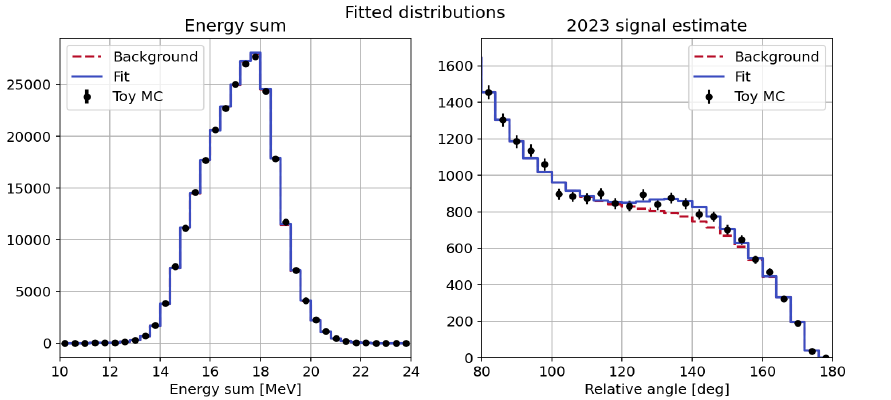
\includegraphics[width=0.9\linewidth]{Figures//X17//Likelihood/examples-binned.png}
            \caption{The binned likelihood fit of a ToyMC sample. It uses 2-dimensional PDFs for $E_{sum}$ and $\theta_{rel}$, presenting ToyMC data (black), the best fit (blue), and summed background PDFs (red).}
            \label{fig:X17:binnedexample}
        \end{figure}
        
\paragraph{Tests}
Many tests are ongoing, like comparing estimators from unbinned and binned likelihood analyses on 500 ToyMC samples, with the second being >50 times faster. 
The different `options' are also tested, revealing option \textbf{D} consistently yields a signal compatible with zero. 
The parametrization for Esum EPC PDFs, dictated by the limited MC production, seems to tend to an overpopulation in background yield. 
The current strategy also lacks consideration for possible correlations between energy sum and relative angle and more tests are needed with final MC production. 

\paragraph{CL estimate}
The distribution of $\lambda_{LR}$ is computed on a $15 \times 15$ grid between 0 and 900 average X17 events and between 15 MeV/c$^2$ and 18.15 MeV/c$^2$ X17 mass. 
For each point in the grid, the ToyMC generation and fitting was performed for 1 h. 
This delivered an inhomogeneous number of ToyMCs produced per point on the grid as the convergence time depends on the strength of the signal. 
Each point in the grid has a generated statistics ranging between $\sim 130$ and $\sim 350$ ToyMCs. 
To compute the CLs, the likelihood on the data sample, which is in this case a reference ToyMC sample, is profiled in the grid points and the $\lambda_{LR}$ is computed. 
For each grid point, the $\lambda_{LR}$ is ranked giving the local CLs. 
The procedure is then repeated 100 times by resampling the dataset and computing the profile likelihood for each iteration for different values of the average X17 yield. 
The median of the upper and lower limits and of the best-fit estimates are studied as a function of the average X17 yield. 
Such estimates depend on the template used, resulting in a bias on the best fit and on the quoted limits. 
The bias is visible, leading to a median yield of 400 X17 events for a scenario where the true value is 450. 
The corresponding plots are in Fig.~\ref{fig:X17:likelihood:CL}.

\begin{figure}
    \centering
    \subfloat[The profile likelihood (left) and the local p-value (right) estimated with Wilks’ theorem, for 500 X17, are shown. The solid/dashed black lines shows the 90\%/68\% p-value levels.]{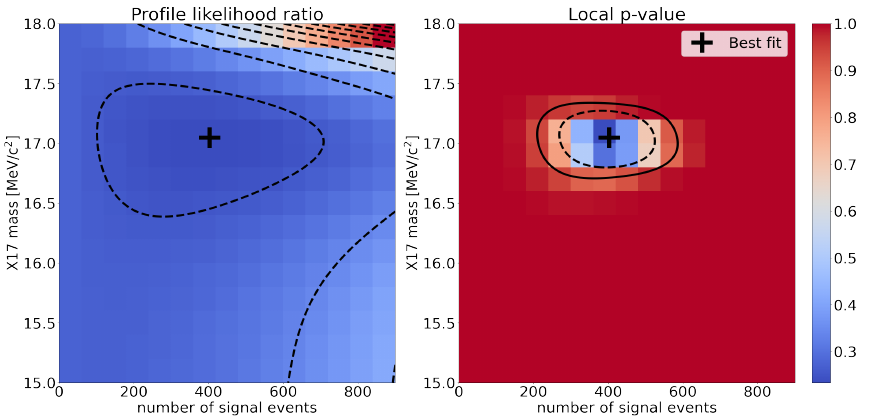
\includegraphics[width=0.9\textwidth]{Figures/X17/Likelihood/likelihood_profile_tests.png}}{}
    \subfloat[FC construction in the ideal statistics scenario for 500 X17. On the right, a cubic spline interpolation is shown. The solid black line shows the 90\% CL belt. By reducing the statistics of the EPC templates by a factor 10, the limits on the X17 yield increase by 14\%, and the limits on the X17 mass increase by 11\%]{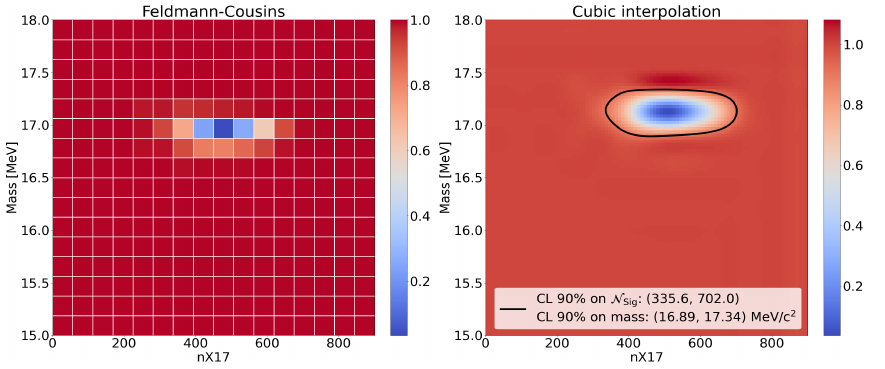
\includegraphics[width=0.9\textwidth]{Figures/X17/Likelihood/likelihood_FC_tests.png}}{}
    \subfloat[Median 90\% CLs and best fits expected as a function of the true X17 yield in the ideal statistics scenarios. The limits are shown both in the estimated X17 yield (left) and mass (right).]{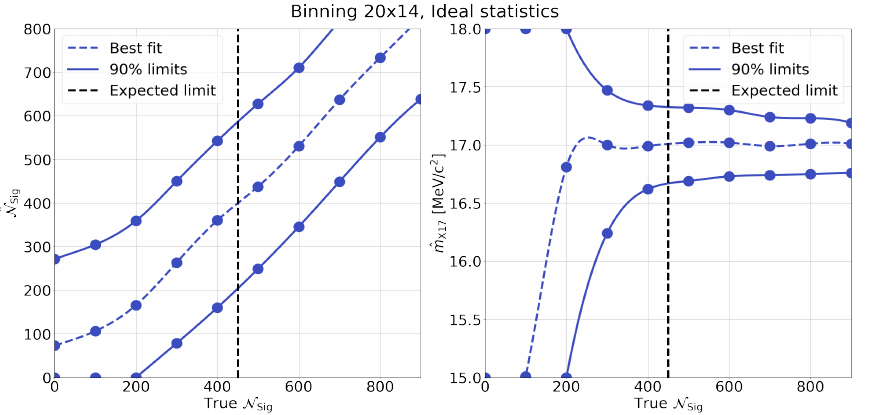
\includegraphics[width=0.9\textwidth]{Figures/X17/Likelihood/likelihood_CL_tests.png}}{}
    \caption{Example of the profile likelihood ratio (a) and of the full FC construction (b) for 500 X17 events in an ideal case. In (c) the median 90\% CLs and best fits expected as a function of the true X17 yield.}
    \label{fig:X17:likelihood:CL}
\end{figure}

\paragraph{Improvements}
Due to the current (and anticipated) limited Monte Carlo statistics, an alternative likelihood approach has been developed. 
In their work, the authors in \cite{X17:likelihood:BB} formulated a binned likelihood for template fits, accounting for the impact of low MC statistics. 
This likelihood combines terms for the observed data ($\mathcal{L}_{data}$) and the template distributions ($\mathcal{L}_{nuisance}$), treating each bin's population as following a Poisson distribution around its true value:
\begin{equation}
    \mathcal{L} = \mathcal{L}_{data} + \mathcal{L}_{nuisance} =
    \sum_{i=1}^n D_i \log (f_i) - f_i + \sum_{i}^{n}\sum_{j}^{m}a_{ij}\log (A_{ij})-A_{ij}
\end{equation}
where $n$ is the number of bins, $m$ the number of populations, $D_i$ the population in the data i-th data bin, $f_i$ the estimated population in the i-th bin, $a_{ji}$ the observed statistics in the j-th MC sample in bin i, and $A_{ij}$ is the estimator of $a_{ji}$.
This approach introduces one nuisance parameter $A_{ij}$ per bin per population, which is used to estimate $f_i$ defining the \textit{population strenght} $p_j$
\begin{equation}
    f_i=\sum_{j=1}^m \frac{\hat{\mathcal{N}}_{data,j}}{\hat{\mathcal{N}}_{MC,j}} A_{ij}= \sum_{j=1}^m p_j A_{ij}
\end{equation}
The maximum of the likelihood is found by solving $\partial_{p_j}\mathcal{L}=0$ and  $\partial_{A_{ji}}\mathcal{L}=0$ analytically or via a minimizer, like MIGRAD.
We will skip the details but this approach would allow us to correct for limited statistics and possible correlations between variables.
This likelihood is currently still under study, with possible changes to implement the analytical (and  faster) minimization.

    \status{review}
    \subsection{Asymmetry and normalization}
        Important aspects to be considered during this search are the different asymmetries expected for the photons resulting from the interaction and the fact that our analysis will require a normalization measurement to keep track of the proton beam intensity.
        For the first task, the obvious choice would have been the XEC but this had two drawbacks: the detector itself is quite limited in extension along the beam direction and it was not always available due to the annealing process described in Sec.~\ref{sec:MEG:XEC}.
        The solution was to use the BGO, described in Sec.~\ref{sec:LH2:BGO}, and crosscheck the results via a dedicated data set collected with the XEC.
        For the normalization, the idea was to install a small NaI crystal below COBRA and use the combined information from this detector, the BGO, and the various measurements of the CW proton current.


        \paragraph{CW stability} The CW is usually used for short periods during CEX calibrations and it is not possible to remote access it.
        On top of it, the only way of measuring the delivered beam current is to momentarily close the beam-shutter, which behaves as a Faraday cup.
        We tried keeping track of the beam intensity during the datataking to cross check this information with the auxiliary detecotr employed for normalization.
        The idea is to have a way of determining, if a drop in rate is observed, if the CW beam had issues or the target.
        A history of the beam current is in Fig.~\ref{fig:X17:CW:current}
        \begin{figure}
            \centering
            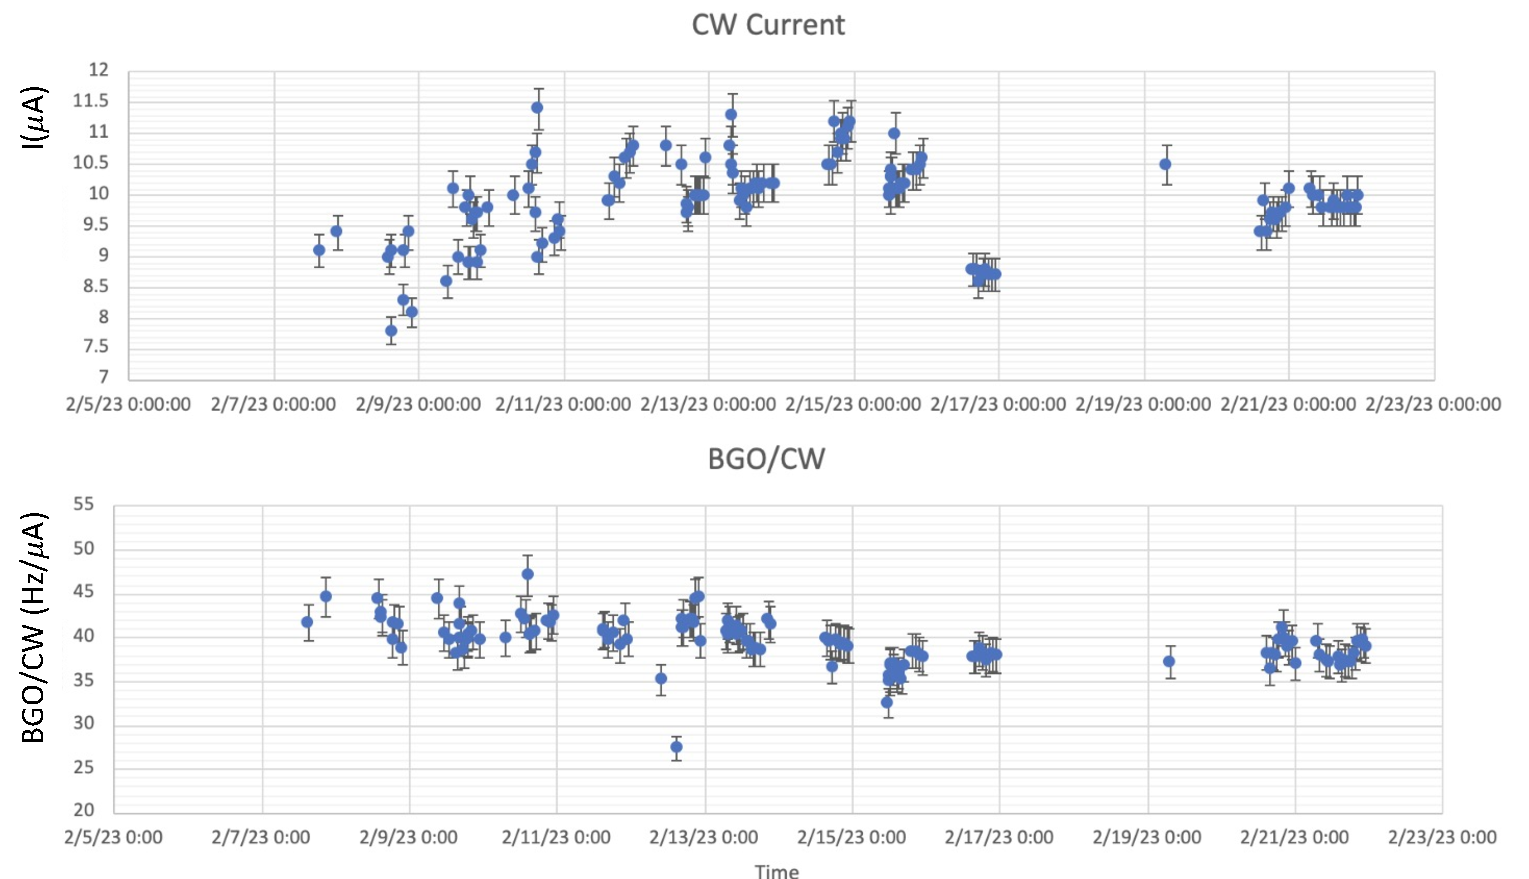
\includegraphics[width = 0.8\textwidth]{Figures/X17/X17_Feb2023/Stability.pdf}
            \caption{History of the CW beam current during X17 data-taking in 2023. In the second plot, the CW current is used to normalize the BGO rate, which is a way to evaluate the stability of the target itself.}
            \label{fig:X17:CW:current}
        \end{figure}

        \paragraph{BGO spectra}
        Here we will not discuss the BGO calibration, which is described in App.~\ref{ch:BGO}.
        The first test was to see if the rotation of the target holder of \SI{90}{\deg} would affect the $\g$ spectra. 
        This could be the case because of the different position of the copper ring holding the target.
        The BGO spectra in the `X17' and the `rotated' position are shown in Fig.~\ref{fig:BGO:rotated} and no substantial difference was found.
        From the width of the \SI{17.6}{MeV}, which is very narrow ($\Gamma=\SI{11}{keV}$), we can extract the BGO energy resolution to be $\sigma_{BGO} \approx 3.1\%$.
        When comparing two subsequent \SI{500}{keV} and \SI{1080}{keV} datasets, we found the two peaks closer than the expected \SI{500}{keV}.
        In practice, the \SI{18.15}{MeV} is at a lower energy and this discrepancy cannot be justified by the precision of the calibration.
        The spectra are shown in Fig.~\ref{fig:BGO:500vs1080}.
        No definitive hypothesis was made on this behavior.
        The two lines of thought were: either the line generated is not the \SI{18.1}{MeV} resonance or there is some detail missing in the detector setup.
        This point will be discussed later in this chapter after the analysis done on the targets and on the CW beam.
        
        \begin{figure}
            \centering
            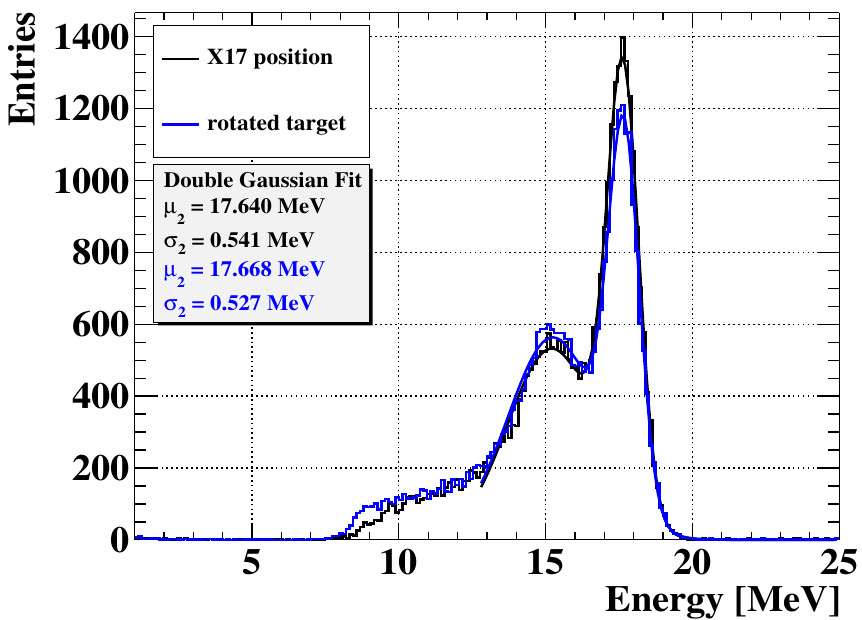
\includegraphics[width=0.9\linewidth]{Figures//X17//BGO/BGO_rotated.png}
            \caption{BGO spectra at $E_p=\SI{500}{MeV}$ for a normal and rotated target. The two spectra are compatible.}
            \label{fig:BGO:rotated}
        \end{figure}

        \begin{figure}
            \centering
            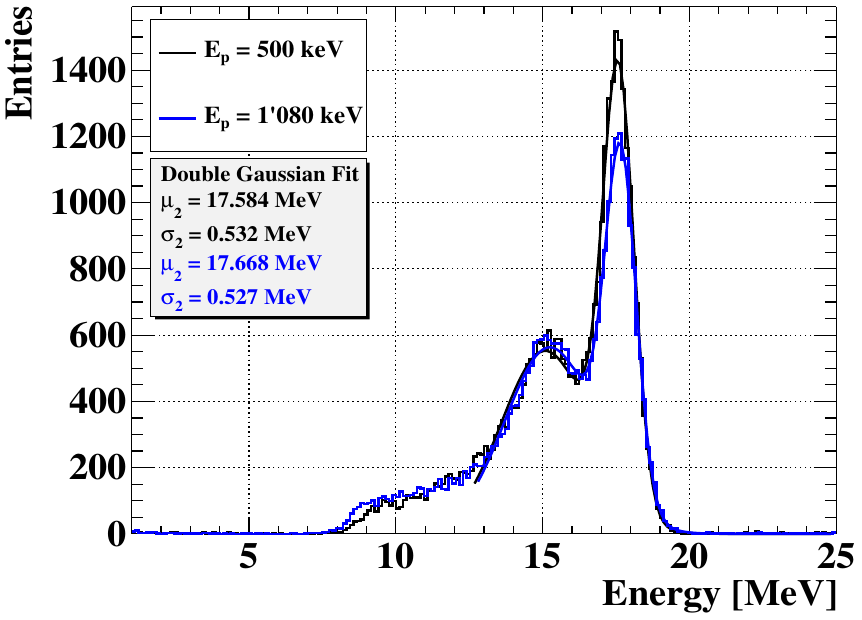
\includegraphics[width=0.9\linewidth]{Figures//X17//BGO/BGO_500vs1080.png}
            \caption{BGO spectra taken at $E_p=\SI{500}{MeV}$ (Black), and $E_p=\SI{1080}{MeV}$ (Blue) on LIPON. The second spectrum should be peaked at \SI{18.15}{MeV} (+\SI{500}{keV}) but is not. The \SI{17.6}{MeV} line seems to be prevalent.}
            \label{fig:BGO:500vs1080}
        \end{figure}

        
        \paragraph{Xenon Calorimeter} 
        In May 23 data with XEC calorimeter as a gamma detector were taken to study the photon spectra, with a 500 nm thin Lipon photon target.
        Fig.~\ref{fig:xecspectrum} shows the photon spectrum taken at different proton energies. As already noticed in the BGO, the two Be(17.6) and Be(18.1) lines don't appear to be separated.
        Another puzzling feature is the relative height of the 15 and 18 MeV peaks.
        Looking at the cross-section in Fig.~\ref{fig:X17:resonance}, one would expect the relative height of the resonance to vary differently.
        
        \begin{figure}[]
            \centering
            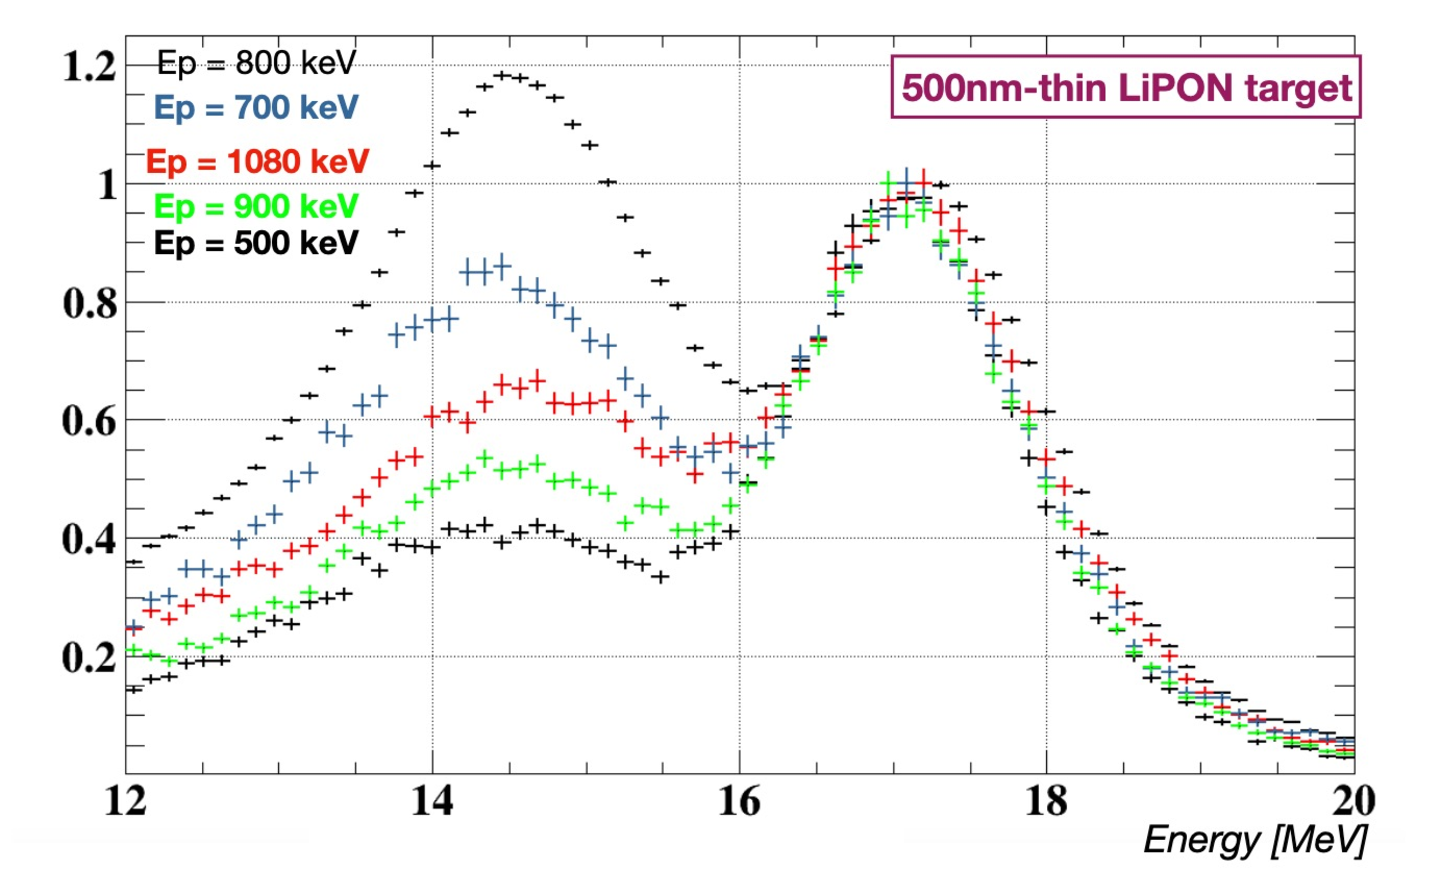
\includegraphics[width = 0.8\textwidth]{Figures/X17/X17_XEC_2023.pdf}
            \caption[X17: XEC data in May 2023]{Photon spectrum measured by XEC detector in May 2023 at different proton energies with a 500 nm thick Lipon target.}
            \label{fig:xecspectrum}
        \end{figure}

    \status{review}   
    \section{Target studies}
    \label{sec:X17:targets}
        To further understand the results of the preliminary analysis, and to cross-check different hypotheses, a few of the targets were studied by experts at PSI and from Sapienza University of Rome.
        These targets were studied with SAM and EDX measurements and the results, of which an example is shown in Fig.~\ref{fig:X17:target:LiPON:psi}, were in line: the targets were found to be poorly characterized, with thicker than expected and uneven deposit.
        After the analysis done on the target used in Feb. during the data-taking, we asked some colleagues from PSI to produce a different LiPON target.
        The requirement was a target `as big as possible' and with a thickness of \SI{500}{\nano m}.
        The way the machine works made it so that the maximum dimension of the target was a diameter of \SI{1}{cm}.
        Given the setup developed for the target was for bigger substrates we had to improvise ways to hold this new target in position.
        We first tried to hold it between two folded aluminum foils. 
        This system was not satisfactory so we moved to a Cu foil with two parallel cuts to create a `pocket'.
        A picture of the two setups is in Fig.~\ref{fig:X17:target:LiPON:psi} while a picture of the target  is in Fig.~\ref{fig:X17:target:LiPON:psi:burned}.
        \begin{figure}
            \centering
            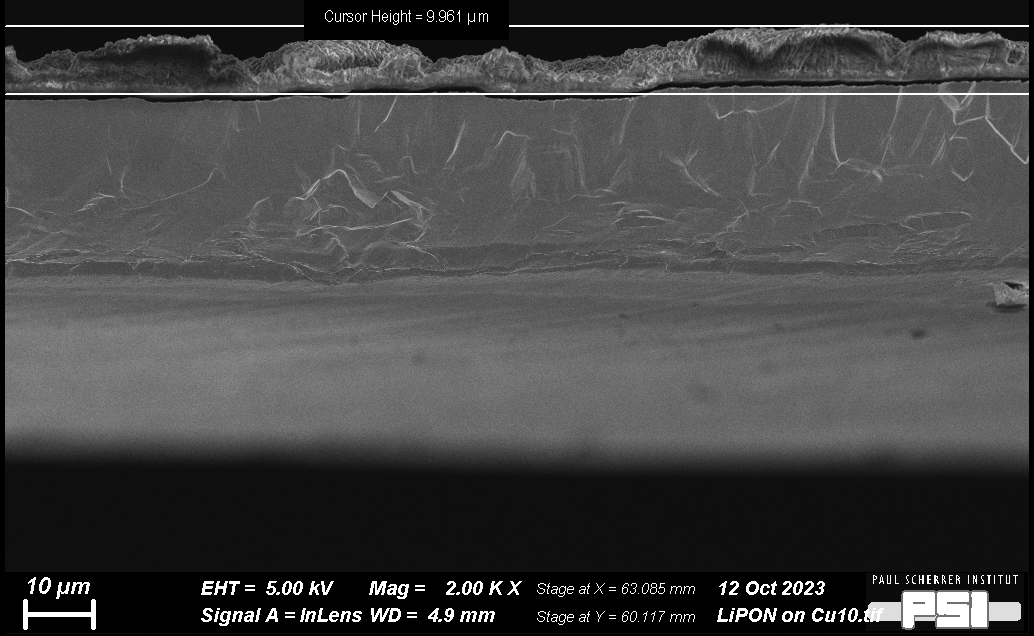
\includegraphics[width = 0.9\textwidth]{Figures/X17/PSI_LiPON_picture.png}
            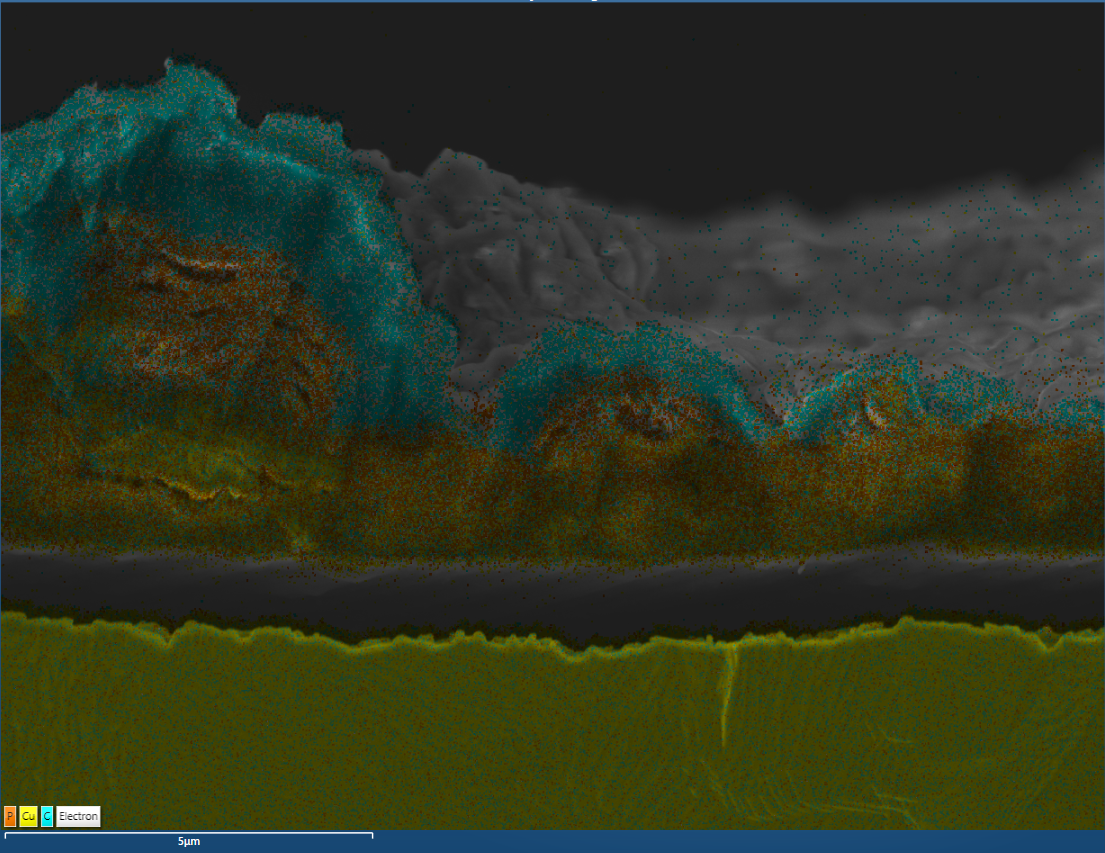
\includegraphics[width = 0.9\textwidth]{Figures/X17/PSI_LiPON-atoms_picture.PNG}
            \caption[SEM EDX LiPON analysis]{SEM and EDX measurement of the \ce{Li3PO4N2} deposit on the Cu substrate. For this particular target, the LiPON deposit was supposed to be \SI{2}{\micro m}. In the top picture, the LiPON rests on the copper substrate. In the bottom picture, the colors highlight the different atoms: Cu-yellow, P-orange, C-cyan. The presence of carbon is linked to the oxidation of the material, creating \ce{LiPO4}. The lamination between LiPON and Cu was attributed to the cutting procedure for the analysis.}
            \label{fig:X17:target:LiPON:psi}
        \end{figure}  

    \status{review}
    \subsection{Al and Cu Data-taking} 
        The data taken with the two different supports (Al and Cu) are confronted in Fig.~\ref{fig:X17:2023:AlCu} for both \SI{500}{keV} and \SI{1080}{keV} protons: for the lower energy we see no difference, the only line excited is the expected resonance at $E_p=\SI{440}{keV}$; for the higher energy a new line appears for the Al. This line demonstrates the energy of the incoming beam to be \SI{1}{MeV}.
        Looking at the sample with the Cu support at the two energies we would expect a shift of \SI{500}{keV} in the peak position. As in the previous data-taking, the shift found is much smaller (see Fig.~\ref{fig:X17:2023:Cu:shift}). Performing a fit with two Gaussians in the expected positions we can evaluate the rough estimate of the two components. The result is a small percentage of the \SI{18.1}{MeV}, around $\sim6\%$.

        \noindent
        The results of these tests highlighted two things: the energy of the CW machine is reliable; the old target seems to not be the (only) cause of the reduced shift in energy at \SI{1080}{keV}.
    
    \begin{figure}
        \centering
        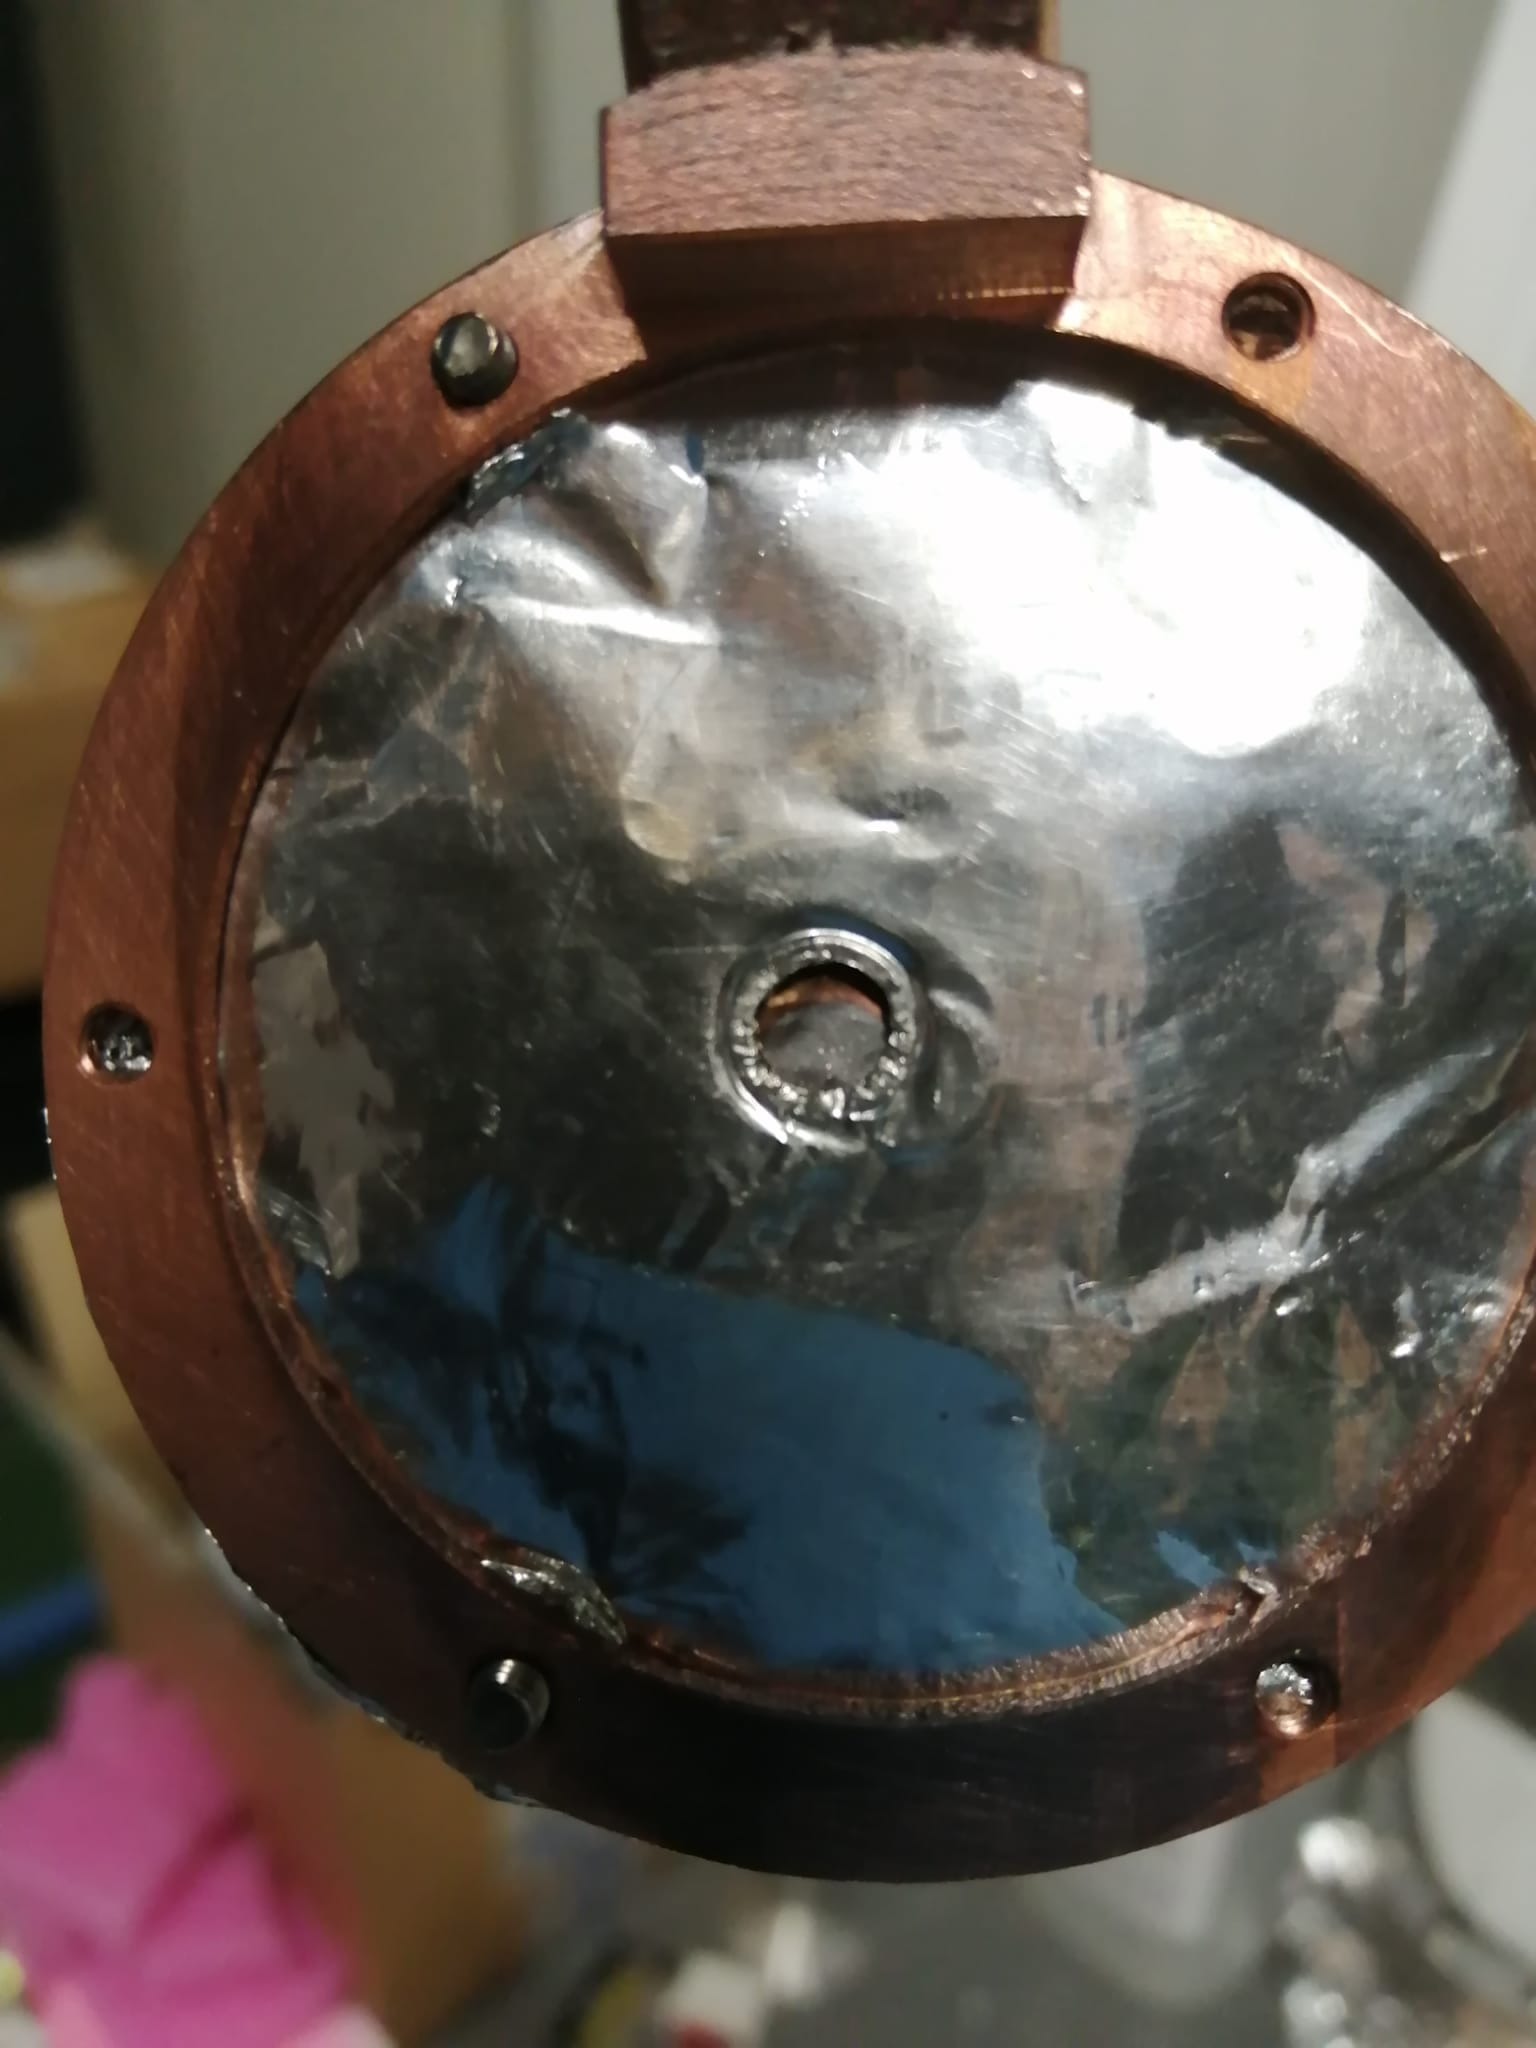
\includegraphics[width = 0.4\textwidth]{Figures/X17/Dec2023/X17_Dec2023_AlTarget.jpeg}
        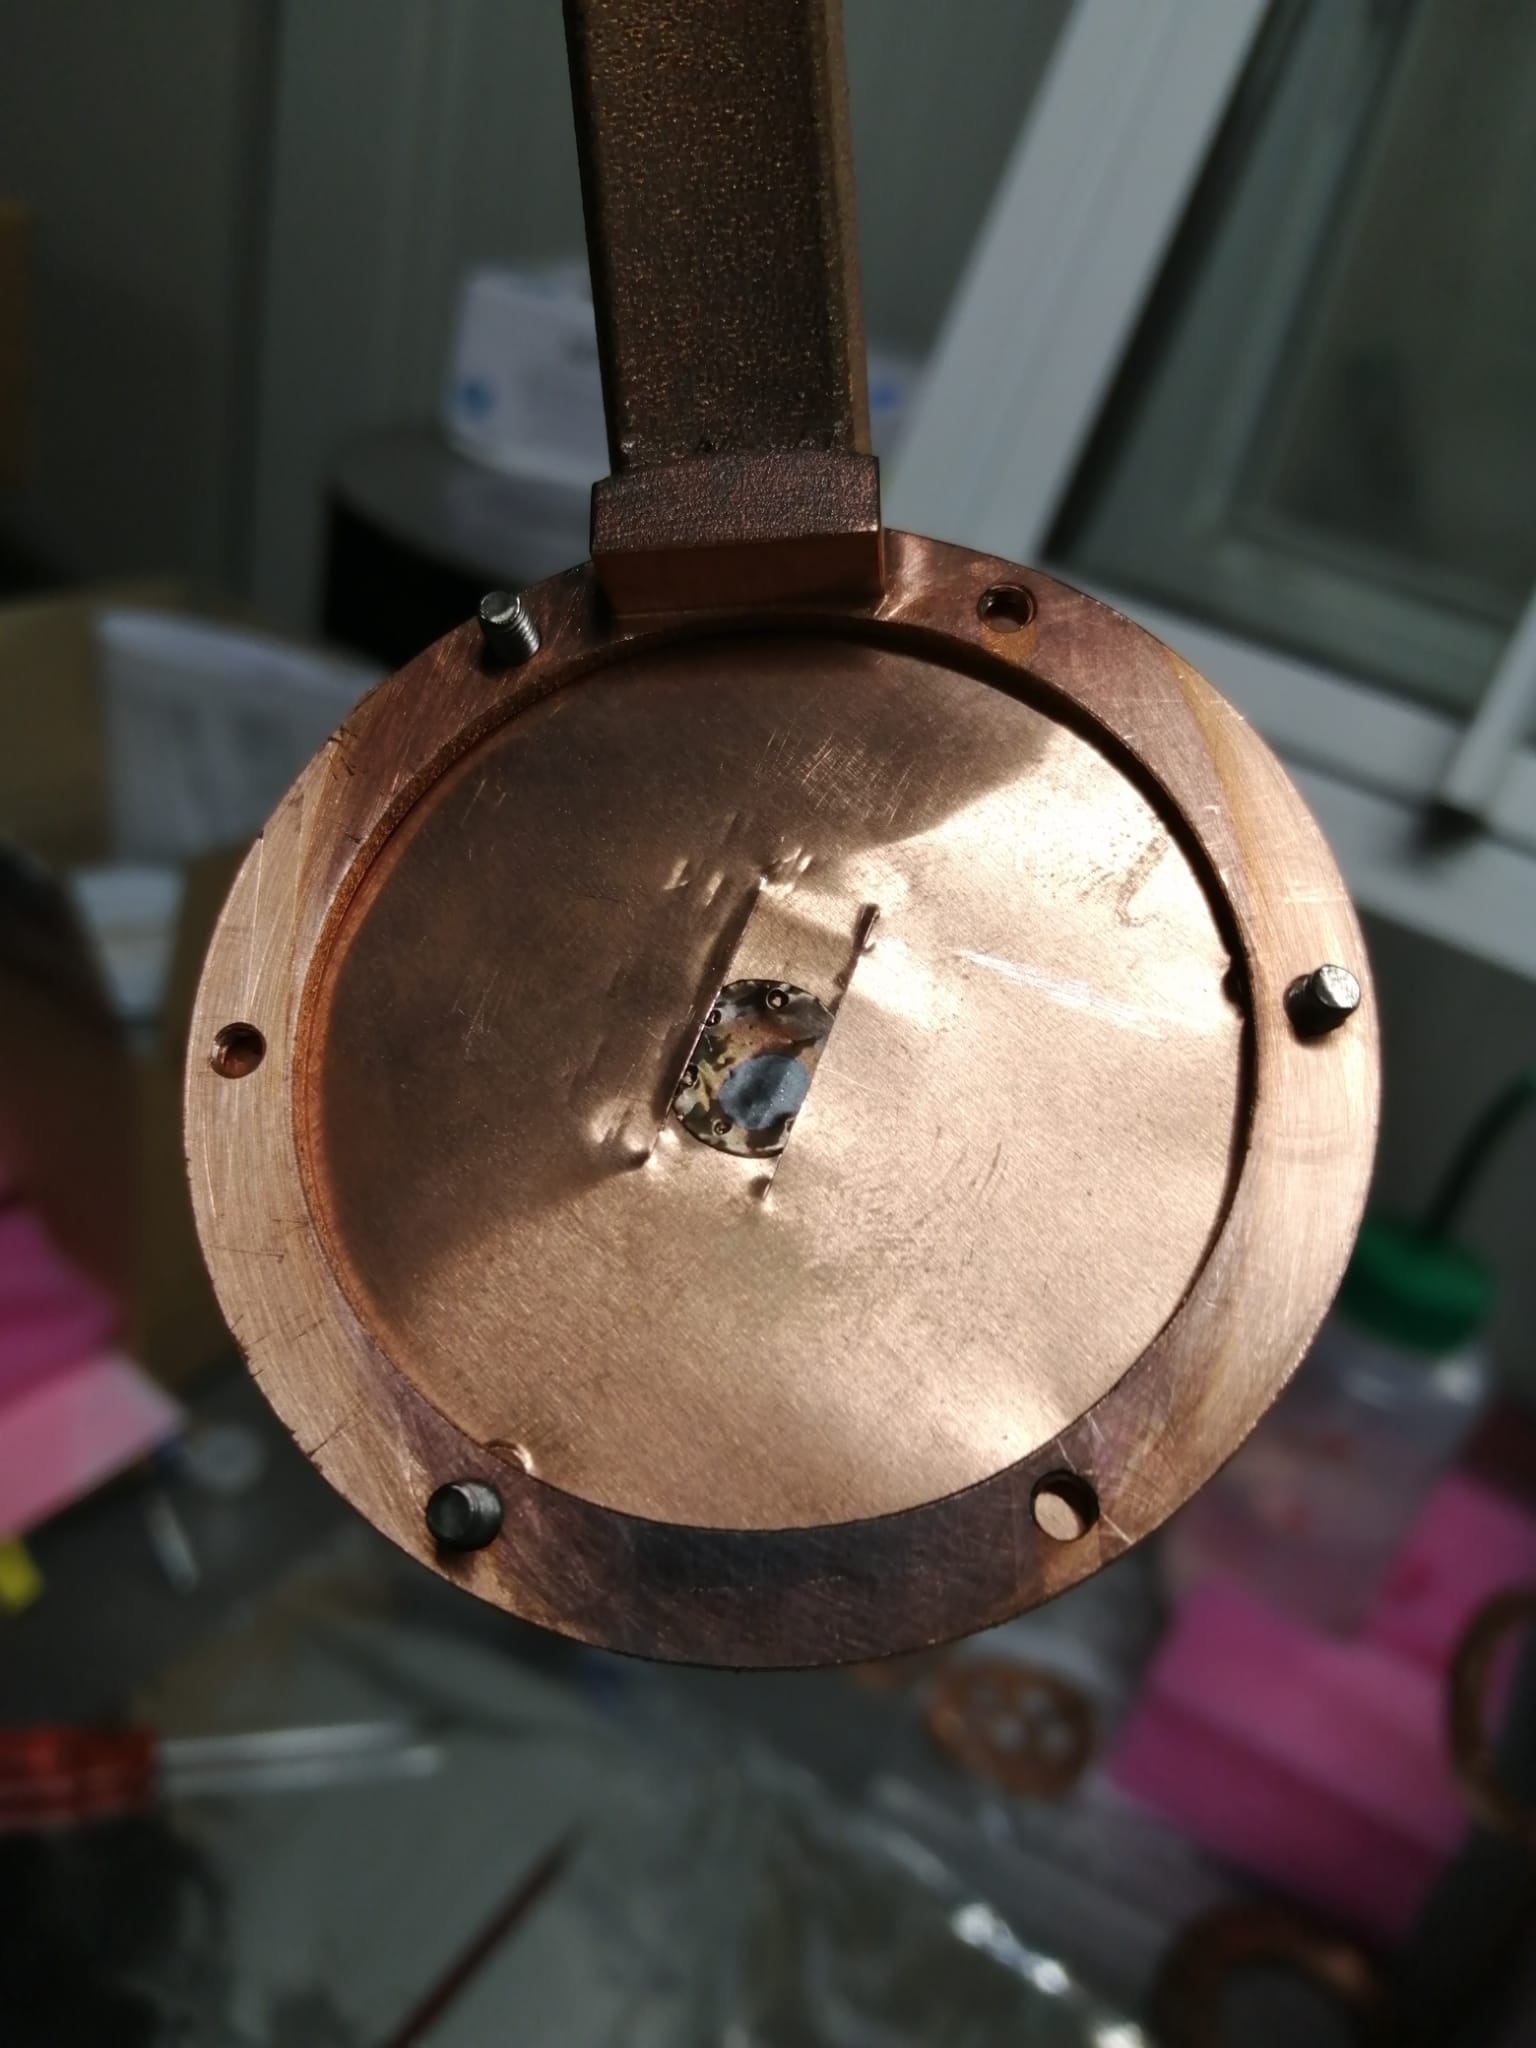
\includegraphics[width = 0.4\textwidth]{Figures/X17/Dec2023/X17_Dec2023_CuTarget.jpeg}
        \caption[X17: Small LiPON target setup]{Two different ways to hold the small LiPON sample given to us by the PSI colleagues. We first tried to hold it in place with folded aluminum foils. We later realized this was not the optimal solution given the spectrum produced by protons on Al. We then moved to a cleaner Cu setup.}
        \label{fig:X17:target:LiPON:psi}
    \end{figure}
    \begin{figure}
        \centering

        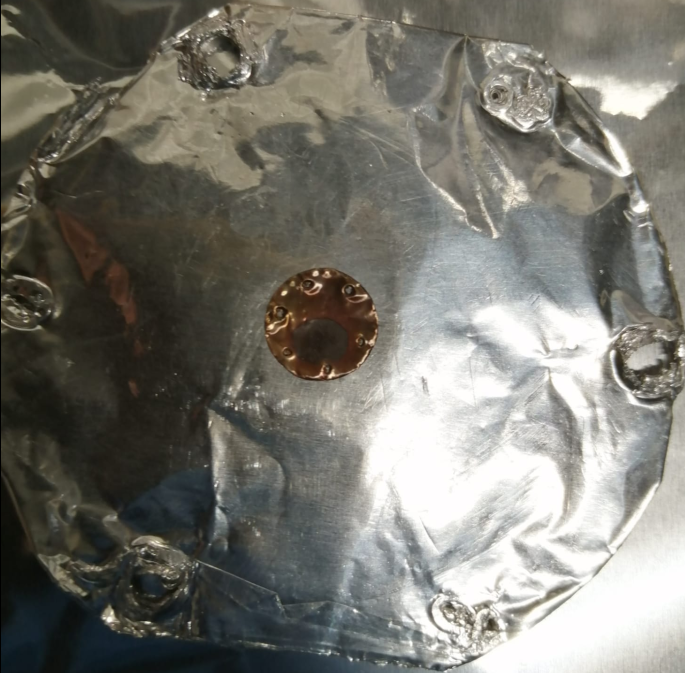
\includegraphics[width = 0.4\textwidth]{Figures/X17/Dec2023/X17_Dec2023_AlTarget_burned.png}
        \caption[X17: Small LiPON target]{Here is a picture of the target itself after two days of data-taking at 5 and \SI{10}{\micro A}. The dark spot marks the position on which the beam was impinging.}
        \label{fig:X17:target:LiPON:psi:burned}
    \end{figure}       

    \begin{figure}
        \centering
        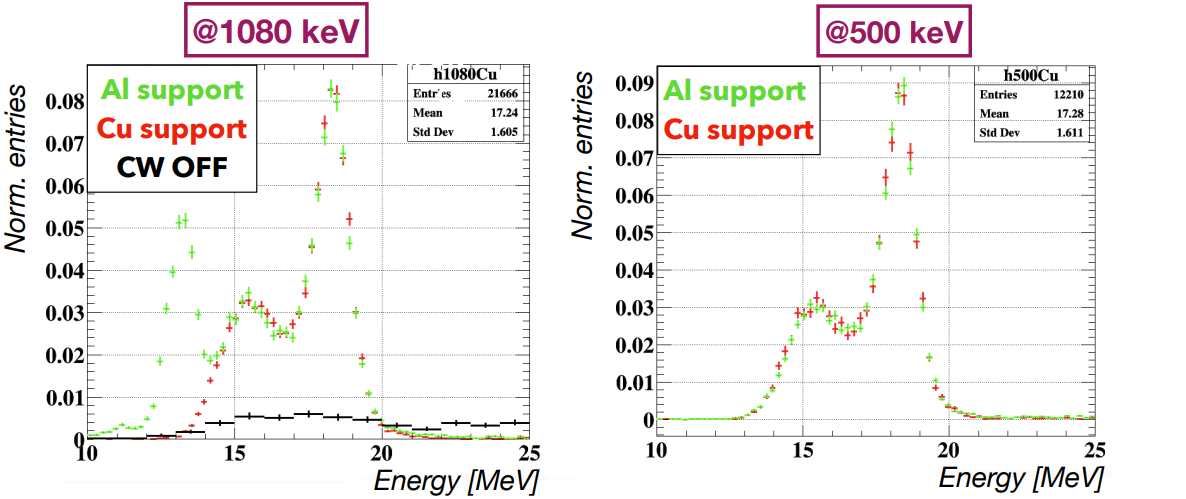
\includegraphics[width = 0.9\textwidth]{Figures/X17/Dec2023/X172023_Al_Cu.png}
        \caption[X17: Al and Cu support spectra]{The data from two supports (Al and Cu) were compared for \SI{500}{keV} and \SI{1080}{keV} protons. At the lower energy, no difference was observed; only the expected resonance at $E_p=\SI{440}{keV}$ was detected. However, at the higher energy, a new line appeared for Al, indicating the energy of the incoming beam.}
        \label{fig:X17:2023:AlCu}
    \end{figure}


    \begin{figure}
        \centering
        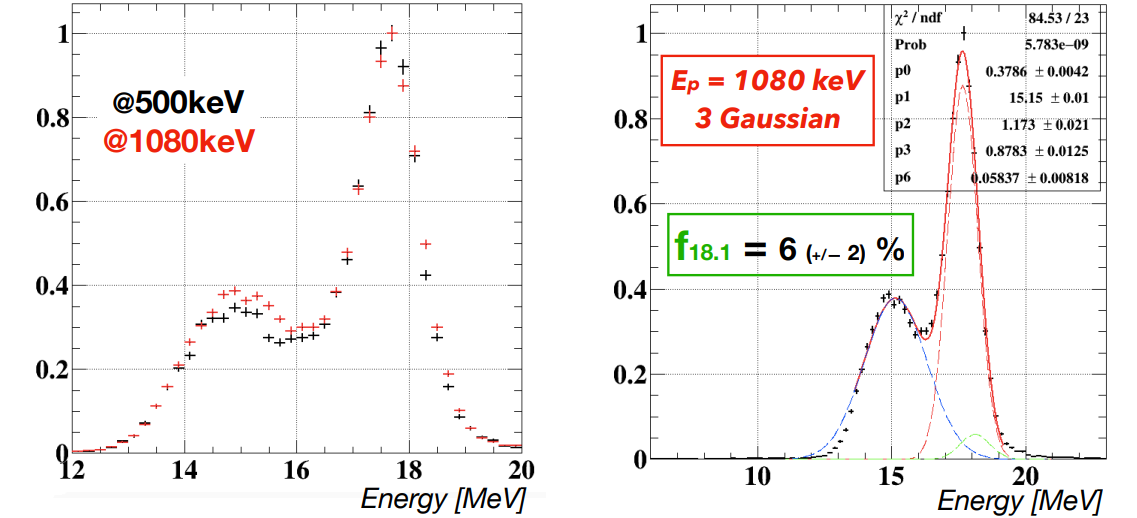
\includegraphics[width = 0.9\textwidth]{Figures/X17/Dec2023/X172023_energy_shift.png}
        \caption[X17: Cu support spectra at 500 and 1080 keV]{Examining the sample with Cu support at both energies, we anticipated a peak position shift of \SI{500}{keV}. However, the observed shift was significantly smaller. By fitting two Gaussians at expected positions, we estimated the two components to be approximately $\sim6\%$ of the \SI{18.1}{MeV}.
}
        \label{fig:X17:2023:Cu:shift}
    \end{figure}

    \status{review}
    \section{Beam studies: Jan 2024}
    \label{sec:X17:H2+}
        After the analysis of the different targets and the small data-taking at the end of 2023, we realized the problem may lay in the proton beam produced by the CW.
        The option of the beam not being at the expected energy was already discarded, for example by the peak measured at $\SI{11}{MeV}$ using aluminum to hold the target.
        The point was that, while producing mainly \ce{H1+}, the machine produces also \ce{H2+} and \ce{H3+}.
        The relative fraction of the different species is roughly $0.7:0.25:0.05$, meaning the fraction of \ce{H2} is non-negligible.
        Having this specie the same $\SI{1}{MeV}$ energy as the protons, when interacting with the target could split, creating  $\SI{500}{keV}$ protons.
        These particles would interact with the Lithium in the much higher resonance, generating the measured \SI{17.6}{MeV} line. 
    
        \status{review}
        \subsection{Collimator and beam studies}
        After mounting the quartz crystal, used already for the beam-tuning in Sec.~\ref{sec:X17:beamtuning}, as close as possible to the CW source ($\approx \SI{2}{m}$) it was possible to see the position of the two beam spots.
        Assuming the brighter one was the one generated by the protons, it was possible to mount a temporary copper collimator to stop the second component of the beam.
        The beam blocker normally functions also as beam current measurement. 
        This system is not designed for that and the occasion was taken to install a Faraday cup and compare the two measurements. 
        By measuring the current with both devices, with and without a collimator, and at different COBRA magnetic fields, it is possible to evaluate the fraction of \ce{H1^+} and \ce{H2^+} reaching the target. 
        The results are shown in Tab.~\ref{tab:X17:beam} and indicate $\sim70\%$ of the beam is \ce{H1^+}.
        An example of the plot used for such a study is in Fig.~\ref{fig:X17:H2+}.\\

        \noindent
        Unfortunately, we experienced a problem similar to what was described in Sec.~\ref{sec:cw:machine}. 
        The machine started sparking at $V>\SI{800}{V}$, meaning that these studies could not be conducted at \SI{1080}{keV} and no further data taking was possible in Feb. 2024.
        The fault seems to be the condition of the \ce{SF6} in the machine but further investigation is ongoing and new \ce{SF6} is on the way to PSI.

        \begin{table}[]
            \centering
            \begin{tabular}{c|c|c}
                \hline
                COBRA & Collimator & Faraday Cup / Beam shutter \\
                \hline
                \hline
                OFF & no & 0.736 \\
                OFF & yes & 0.518 \\
                \SI{0.15}{T} & no & 0.748 \\
                \SI{0.15}{T} & yes & 0.530 \\
                \hline
            \end{tabular}
            \caption{Summary of the measurements on the CW beam}
            \label{tab:X17:beam}
        \end{table}

        \begin{figure}
            \centering
            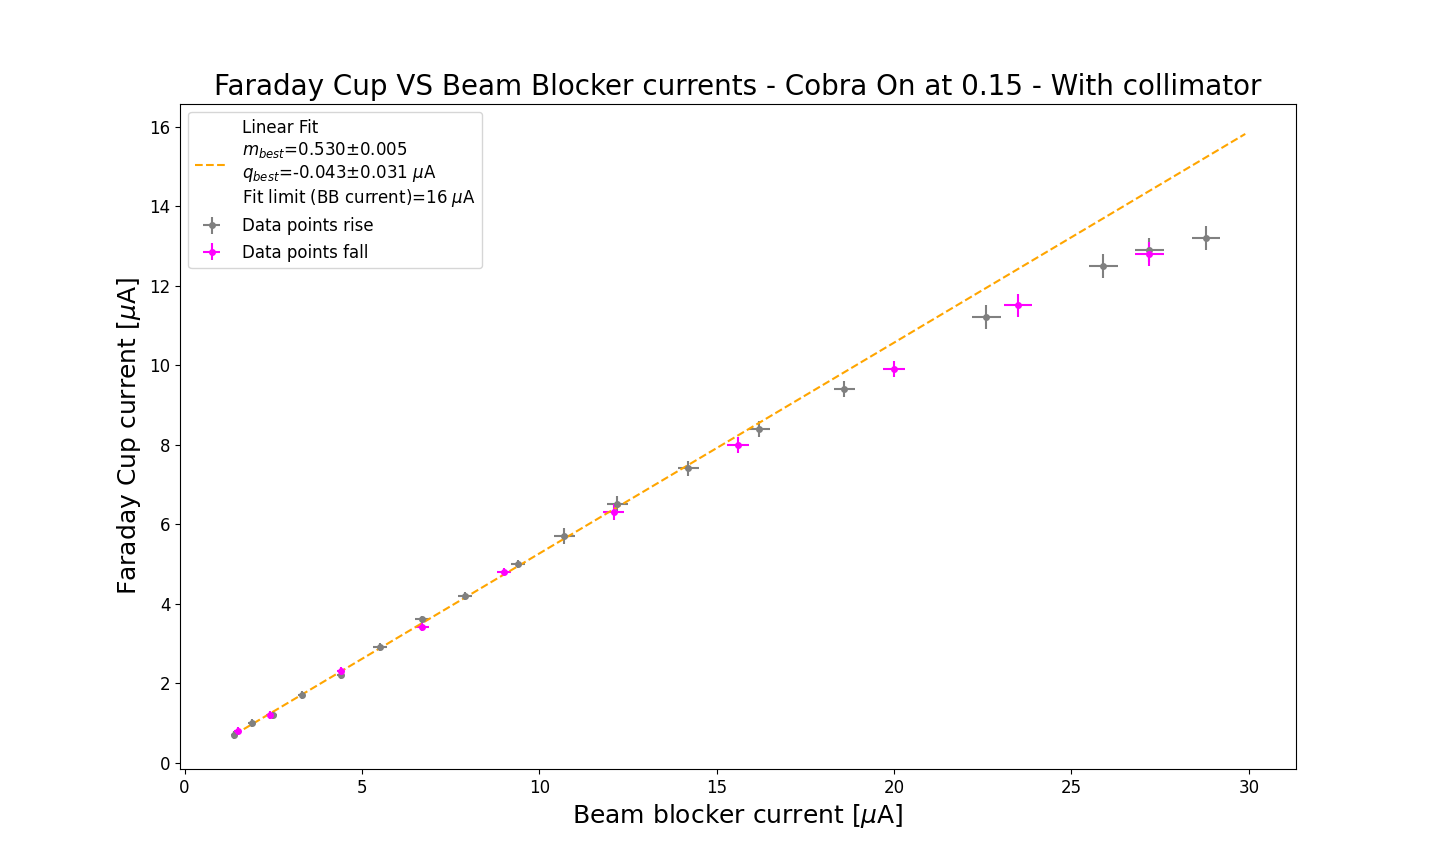
\includegraphics[width = \textwidth]{Figures/X17/H2+/Faraday_Cup_VS_Beam_Blocker_currents_-_Cobra_On_at_0.15_-_With_collimator.png}\\
            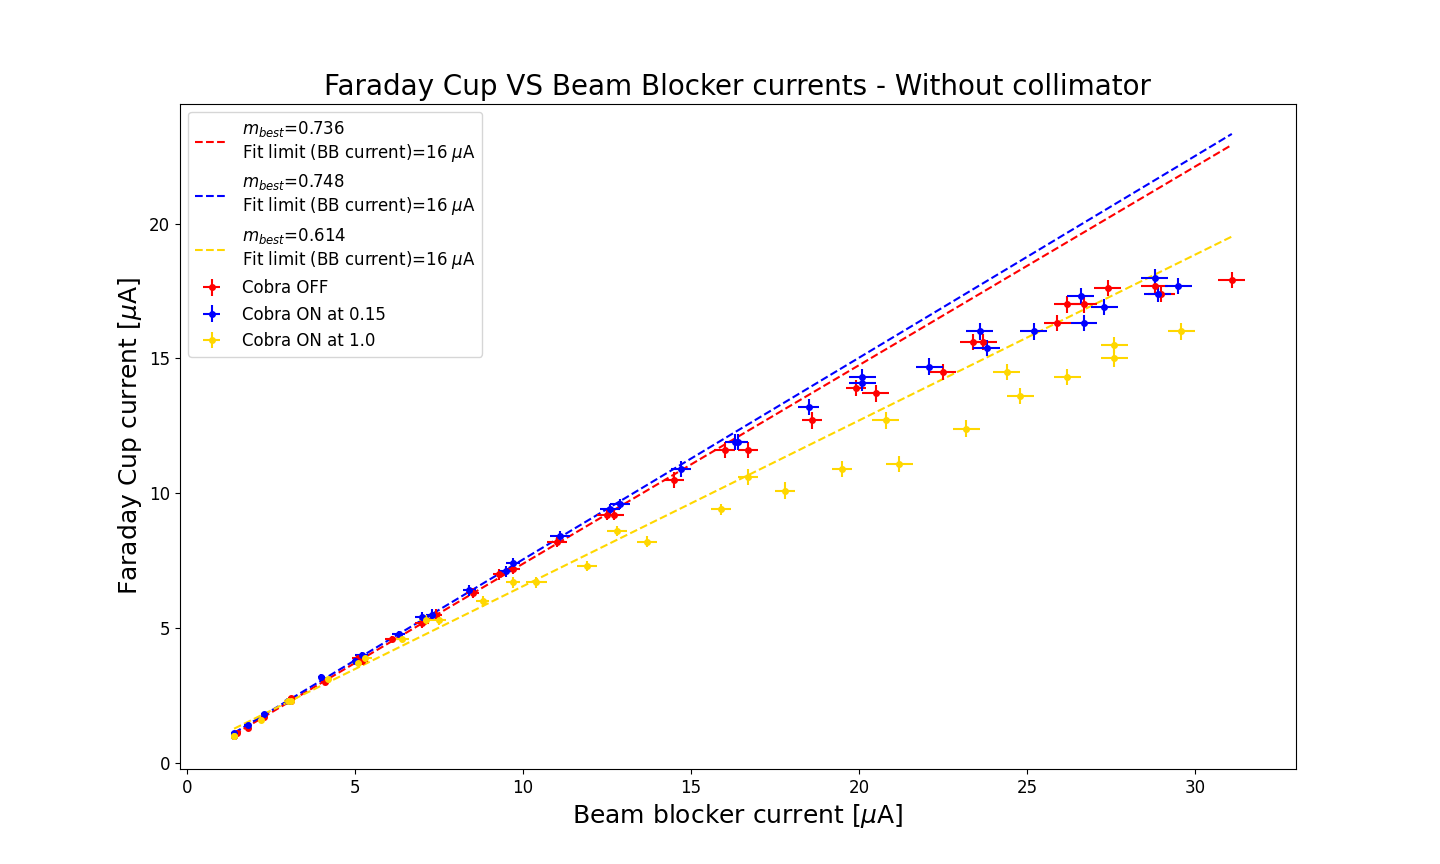
\includegraphics[width = \textwidth]{Figures/X17/H2+/Faraday_Cup_VS_Beam_Blocker_currents_-_Without_collimator.png}
            \caption{Example of the data taken in Feb. 2023 to study the CW beam. The top picture shows the dependence of the current measured with the Faradey Cup with collimator as a function of the Beam Blocker current with COBRA at 15\%. The bottom plot shows the same plot with no collimator but with different magnetic fields.}
            \label{fig:X17:H2+}
        \end{figure}

\status{review}
\section{Results and conclusions}
    This chapter was dedicated to the X17 search with the MEG II apparatus.
    After a summary of the anomaly under study we saw how the search is ongoing in MEG II, with details on the analysis. 
    Unfortunately, the data of 2023, while still of interest, are dominated by the \SI{17.6}{MeV} line instead of the \SI{18.1}{MeV} due to the target and/or \ce{H2+} CW beam component. 
    I had an active role in all preparations and data-taking and played I marginal role in the analysis, particularly in the development of the likelihood analysis framework and the BGO calibration procedure.\\
    
    \noindent
    Regarding the data-taking campaign of 2023, the MC simulation accuracy is under investigation in sidebands, with ongoing MC production. 
    We plan to address the limited MC statistics, due to resource constraints, implementing the Beeston-Barlow likelihood, discussed in Sec.~\ref{sec:X17:likelihood}. 
    The expected sensitivity on the 2023 data is 272(4) X17 events, compared to 450 by ATOMKI.
    The estimated significance of an anomaly akin to ATOMKI's measurements is 3.36$\sigma$; a 4.27$\sigma$ significance could be reached with a tenfold increase in EPC MC statistics.\\
    
    \noindent
    The collaboration plans to have another data-taking focusing on the \SI{18.1}{MeV} line changing the target, as discussed in Sec.~\ref{sec:X17:targets}, and removing the \ce{H2+} from the CW beam, as discussed in Sec.~\ref{sec:X17:H2+}. 
    These two improvements should give a sample that is purer and with a higher expected sensitivity.

\status{started}
\printbibliography[
    heading = bibliographychapter,
    title=Bibliography on X17
]

\end{refsection}
